\documentclass[10pt, conference, letterpaper]{IEEEtran}
\usepackage[margin=1mm]{caption}
\usepackage{graphicx}
\usepackage{subfigure}
\usepackage{url}
\usepackage[american]{babel}
\usepackage[utf8]{inputenc}
\usepackage{tikz}
\usepackage{amsmath}
\usepackage{amssymb}
\usepackage{times}
\usepackage{cite}
\usepackage{color}
% \usepackage[T1]{fontenc}

%\makeatletter
%\newif\if@restonecol
%\makeatother
%\let\algorithm\relax
%\let\endalgorithm\relax
% \usepackage[lined,ruled,linesnumbered]{algorithm2e}
\usepackage[ruled,linesnumbered]{algorithm2e}

\newcommand{\ed}[1]{\textbf{[[#1]]}}
\newcommand{\dtrack}{\textsc{dtrack}}
\newcommand{\rmprt}{{Re\-map\-Rou\-te}}
\newcommand{\figstr}{Fig.}
\newcommand{\figstrs}{Figs.}
\newcommand{\secstr}{Sec.}
\newcommand{\secstrs}{Secs.}
\newcommand{\tabstr}{Tab.}
\newcommand{\tabstrs}{Tabs.}
\newcommand{\paragraphnd}[1]{\vspace{2mm}\noindent\textbf{#1}}
\renewcommand{\paragraph}[1]{\vspace{2mm}\noindent\textbf{#1.}}

\newcommand{\blue}[1]{{\color{blue}#1}}

\hyphenation{re-map-rou-te}
\hyphenation{Re-map-Rou-te}

\sloppy

\title{Local Remapping of Internet Path Changes}

\newfont{\cunhaemail}{phvr8t at 8.5pt}

% \numberofauthors{1}

% \author{
% \noindent{}
% \begin{tabular}{cccc}\\
% \vspace{0.3em}
% \Large{\'{I}talo Cunha} &
% \Large{Renata Teixeira} &
% \Large{Darryl Veitch} &
% \Large{Christophe Diot} \\
% \affaddr{Universidade Federal} &
% \affaddr{Inria} &
% \affaddr{Dept. Elec. and Elec. Eng.} &
% \affaddr{Technicolor}\\
% \affaddr{de Minas Gerais} &
% &
% \affaddr{University of Melbourne} &
% \\
% \cunhaemail{cunha@dcc.ufmg.br} &
% \cunhaemail{renata.teixeira@inria.fr} &
% \cunhaemail{dveitch@unimelb.edu.au} &
% \cunhaemail{christophe.diot@technicolor.com}
% \end{tabular}
% }

\author{Paper \#000\vspace{2cm}}

%Italo Cunha\\
%        \affaddr{Universidade Federal de Minas Gerais}\\
%        \cunhaemail{cunha@dcc.ufmg.br}\\
%\alignauthor
%Renata Teixeira\\
%\alignauthor
%Darryl Veitch\\
%\alignauthor
%Christophe Diot\\
%        \affaddr{Technicolor}\\
%}

\begin{document}

\maketitle

\selectlanguage{american}

\begin{abstract}
%
A number of systems rely on traceroute to track a large number
of Internet paths as they change over time.  Our previous work designed
\dtrack{}, a system that optimizes probing to track Internet path
changes.  \dtrack{} only remaps a path, i.e., probes every hop from the
source to the destination of the path, after it detects that the path
has changed.  This paper shows that such complete remapping is
inefficient, because most path changes are localized in a few hops of a
path.  We develop a new version of DTrack with local remapping, which
just probes the (often few) hops that have changed.  Our evaluation with
trace-driven simulations and in a PlanetLab deployment shows that local
remapping reduces by 73\% the number of probes issued during remapping
when compared with complete remapping.  Yet, local remapping has little
impact on the accuracy of inferred paths.
%
\end{abstract}

\section{Introduction}
\label{sec:intro}

A number of distributed services and applications need to measure
Internet paths to maintain an up-to-date view of the underlying
infrastructure~\cite{duffield06binary,
dhamdhere07netdiagnoser,kompella07blackholes,
bassett12lifeguard,akamai,skitter}. All these systems use some version
of traceroute to repeatedly measure a large number of Internet paths.
Traceroute sends probes to every hop between a source and a destination,
so the measurement of a single path often requires tens of probes and
takes some seconds~\cite{veitch09balancer}. The number of probes required
to measure a path is even larger if one wants to measure all paths
between a source and a destination when routers perform load
balancing~\cite{veitch09balancer}. For example, discovering a
(multi)path with Paris traceroute, which is a traceroute version that
discovers all paths under load balancing, requires hundreds of probes
and takes tens of seconds~\cite{veitch09balancer}.\footnotemark{}
Because measuring each path takes time, a source cannot measure paths
frequently and as a result it may miss path changes. For instance,
topology mapping systems can take from several minutes to a few days to
measure all required paths~\cite{cunha11fastmapping, sherwood08discarte,
skitter}.  In between measurements, paths may be outdated or
inconsistent.

\footnotetext{
% Given the
% prevalence of load balancing in the Internet~\cite{augustin07},
It is essential to accurately measure paths under load balancing to avoid
traceroute errors and misinterpretation of path
changes~\cite{cunha11fastmapping}.}

Our previous work showed that Internet paths being mostly stable,
measuring all paths at the same frequency wastes probes in paths that
are not changing~\cite{cunha11dtrack}. We developed \dtrack{}, a system
that optimizes probing to track Internet path
changes~\cite{cunha11dtrack}.  \dtrack{} splits the task of tracking
paths into two sub-tasks.  \textit{Path change detection} sends a single
probe per path at any given time, probing more frequently paths that are
more likely to change. \textit{Path remapping} responds to a path change detection
by immediately sending probes to discover all interfaces of the new multipath.
Although \dtrack{} detects twice as many path changes
as traditional probing~\cite{cunha11dtrack}, remapping a path remains
costly.  \dtrack{} simply runs Paris traceroute to remap the entire
end-to-end path. Such complete remapping ensures the accuracy of
inferred paths, but incurs a large probing overhead.

In this paper, we show that complete remapping wastes probes because
most path changes are localized in a few (consecutive) hops of a path
(\secstr~\ref{sec:char}). We build on this observation to develop a more
efficient remapping method for \dtrack{} (\secstr~\ref{sec:remap}).
Given knowledge of the path before the change and the hop where the
change was detected, we first send probes to precisely locate the change and then
just remap the (generally few) hops that have changed. We call this
method \textit{local remapping} as opposed to the complete remapping
originally implemented in \dtrack{}. Local remapping still uses Paris
traceroute's multipath detection algorithm~\cite{veitch09balancer} for
discovering all interfaces at a given hop to guarantee accuracy, but we
no longer have to remap every single hop of the path.

Our evaluation via trace-driven simulations shows that local remapping
reduces the remapping probing cost of 88\% of path changes in our dataset by
more than half, and reduces overall cost by 73\% (\secstr~\ref{sec:sim}).
Local remapping has two  limitations: (i) it may only remap part of the
change when paths change in multiple locations; and (ii)  it does not
work when a path change reorders the interfaces of the path.  We show
that local remapping accurately remaps all changes in a path for 87\%
of path changes and that less than 1\% of path changes reorder hops
(\secstr~\ref{sec:sim}).  We develop a new version of \dtrack{} with
local remapping.  Our evaluation in a PlanetLab deployment shows that
local remapping inferences are identical to those obtained with complete
remapping for 92\% of path changes (\secstr~\ref{sec:deploy}). Yet,
local remapping reduces overall probing cost by 75\% when compared with
complete remapping.
\pagebreak

An early version of this work appeared (in Portuguese) at the Brazilian
Computer Networks and Distributed Systems Symposium~\cite{cunha13remap}.
Here we improve the path change remapping formalism and give an
evaluation with larger data sets.

% If we use the probes we save by using local remapping for detection,
% our new version of \dtrack{} can track \ed{XXX} more path changes than
% the original \dtrack{} with end-to-end remapping and \ed{XXX} more
% changes than traditional probing.

%
%Reducing remapping costs increases the number of probes available for
%topology mapping.  We can use the extra probes to monitor more paths and
%improve network coverage, or we can increase probing frequency and
%improve routing change tracking.  \rmprt{} is another step toward
%building more complete and consistent Internet maps.

%Internet failure identification systems usually require information
%about network routes~\cite{duffield06binary, dhamdhere07netdiagnoser,
%kompella07blackholes, bassett12lifeguard}.  Similarly, content
%distribution networks measure Internet routes to choose the ``best''
%server to answer a request~\cite{akamai}.  These and other systems
%measure routes frequently in an attempt to track routing changes as they
%happen.
%
%Internet route measurements are usually performed with
%traceroute~\cite{veitch09balancer, spring02rocketfuel,
%madhyastha06iplane}, which sends probes to identify a sequence of
%interfaces between a source and a destination.  The bandwidth available
%to send probes is finite.  Route measurements for topology mapping
%require a large number of probes and can take from several minutes to a
%few days~\cite{cunha11fastmapping, sherwood08discarte, skitter}.  It is
%impossible to measure routes frequently enough to detect all routing
%changes without overloading the network.  Thus, Internet topology maps
%may be outdated, or inconsistent as routing changes may occur during the
%measurement process.
%
%Our \dtrack{} system tracks Internet routing changes to keep Internet
%topology maps more up-to-date~\cite{cunha11dtrack}.  \dtrack{} separates
%the tasks of detecting and remapping routing changes.  To detect
%changes, \dtrack{} uses a lightweight probing process that combines two
%main ideas: (1) redirect probes from stable paths, where routing changes
%are unlikely, to unstable paths, where routing changes are more likely;
%and (2) spreading probes uniformly over the network and over time to
%reduce redundant probes.  \dtrack{} keeps a database with the previous
%route observed on each monitored path.  \dtrack{} sends a probe to a hop
%in the path and compares the IP address in the reply with the IP address
%in the previous route.  If the probe reply is incompatible with the
%previous route, e.g., the IP address in the probe reply is not in the
%previous route, a change is detected and the remapping process is
%triggered.
%
%To remap changes, \dtrack{} uses Paris
%traceroute~\cite{veitch09balancer} to measure the current route.  Paris
%traceroute is an improved version of traceroute that identifies routers
%that perform load balancing.  \dtrack{} uses Paris traceroute because it
%is impossible to differentiate routing changes from load balancing
%otherwise~\cite{cunha11fastmapping}.  Currently, \dtrack{} remaps the
%whole path using Paris traceroute.  This approach guarantees correct
%remapping of the current route, but wastes probes as most routing
%changes involve few hops (\secstr~\ref{sec:char}).  In particular, this
%approach ignores two pieces of information available when the remapping
%process begins: the previous route and the hop where the change was
%detected.
%
%In this paper we propose \rmprt{}, a new tool to reduce the cost of
%remapping Internet routing changes (\secstr~\ref{sec:remap}).  Given the
%previous route observed before the change and a hop where a change was
%detected, \rmprt{} strategically sends probes to locate the change and
%locally remap it rather than waste probes on an unnecessary complete
%remapping.
%
%Our evaluation via trace-driven simulations shows that \rmprt{} reduces
%by half the remapping cost of 88\% of routing changes in our dataset
%(\secstr~\ref{sec:sim}).  Remap cost reduction is even larger for routes
%traversing routers that perform load balancing.  RemapRoute's
%optimizations do not work if a previous route measurement is unavailable
%or if a routing change reorders hops (0.9\%), but is otherwise
%statistically equivalent to Paris traceroute (\secstr~\ref{sec:sim}).
%Our evaluation of \rmprt{} in a real deployment confirms our simulation
%results and demonstrates \rmprt{}'s accuracy (\secstr~\ref{sec:deploy}).
%We make the following contributions:
%
%% FIGS 1--3 FROM SEC. 3
%\begin{figure*}[t]
%\begin{minipage}{0.33\textwidth}
%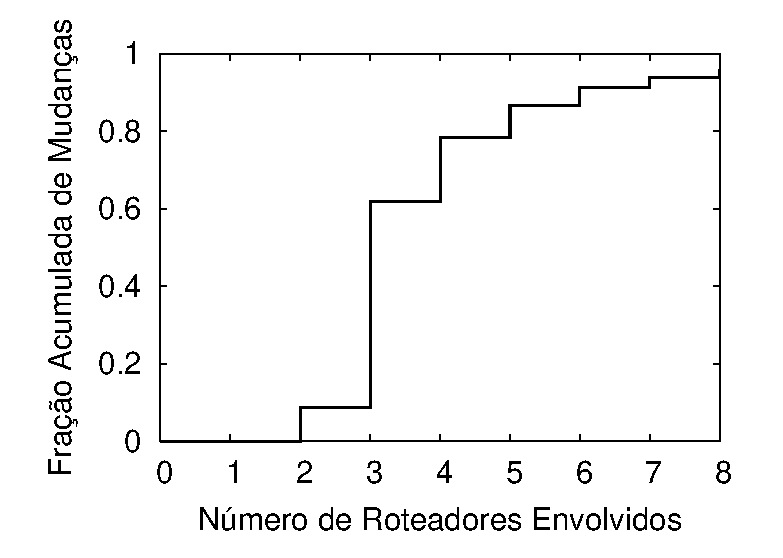
\includegraphics[width=1.05\textwidth]{figs/nrouters.eps}
%\caption{Distribution of the number of hops involved in path changes.}
%\label{fig:char.nrouters}
%\end{minipage}
%\hfill
%\begin{minipage}{0.33\textwidth}
%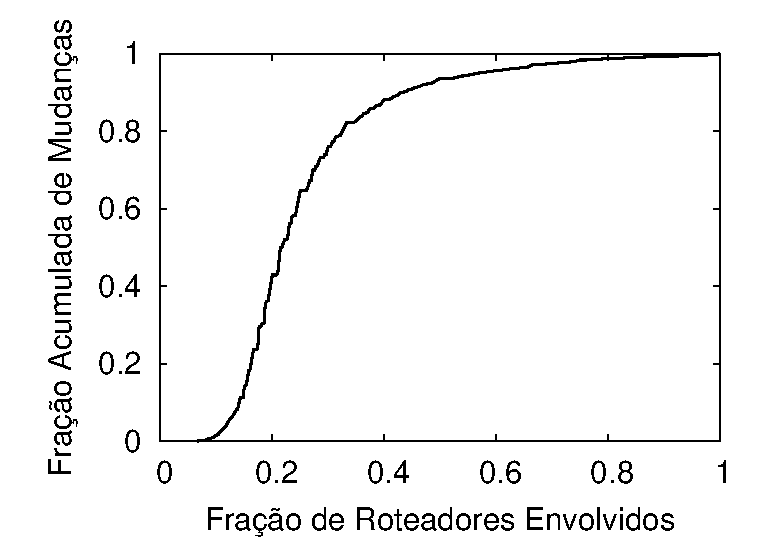
\includegraphics[width=1.05\textwidth]{figs/fracs.eps}
%\caption{Distribution of the fraction of routers involved in path changes.}
%\label{fig:char.fracs}
%\end{minipage}
%\hfill
%\begin{minipage}{0.33\textwidth}
%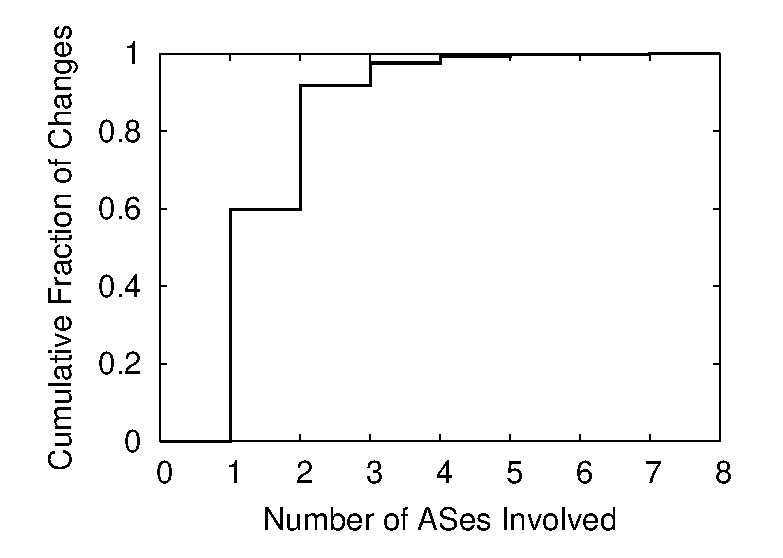
\includegraphics[width=1.05\textwidth]{figs/nasns.eps}
%\caption{Distribution of the number of ASes involved in path changes.}
%\label{fig:char.nasns}
%\end{minipage}
%\end{figure*}
%
%\begin{itemize}
%%
%\item We characterize Internet routing changes and show that they
%usually involve few hops (\secstr~\ref{sec:char});
%%
%\item We propose methods to locate and remap path changes that reduce
%wasted probes (\secstr~\ref{sec:remap});
%%
%\item We show the efficacy of our tool with trace-driven simulations and
%in a real deployment (\secstrs~\ref{sec:sim} and~\ref{sec:deploy}).
%%
%\end{itemize}
%
%Reducing remapping costs increases the number of probes available for
%topology mapping.  We can use the extra probes to monitor more paths and
%improve network coverage, or we can increase probing frequency and
%improve routing change tracking.  \rmprt{} is another step toward
%building more complete and consistent Internet maps.




\section{Definitions and background}
\label{sec:background}

% definition of local change zone acronym
\newcommand{\LCZ}{\ensuremath\mathrm{\textsc{lcz}}}

We follow the same notation as in our previous
work~\cite{cunha11dtrack}.  We use \emph{virtual path} to refer to the
connectivity between a fixed source $s$ and a destination $d$.  At any
given time, a virtual path is realized by the \emph{current route}.
Since routing changes occur, a virtual path is a continuous time process
$P(t)$ which jumps between different routes over time. A \emph{route}
can be \emph{simple}, consisting of a sequence of IP interfaces from $s$
toward $d$, or \emph{branched}, when one or more \emph{load balancing}
routers are present, giving rise to multiple overlapping sequences
(called ``multi-paths'' in \cite{veitch09balancer}).  Thus a route is a
directed graph with interface-labelled nodes.

% \ed{A route can be a sequence that terminates before reaching $d$.
% This can occur due to routing changes (e.g., transient loops), or the
% absence of a complete route to the destination.}

By \emph{hop-set} or \emph{hop} we mean the set of interfaces (one
interface per branch), found at some fixed distance or radius from the
source.  We denote the hop-set at radius $r$ in route $p$ as $p[r]$.
Conversely, for some valid hop-set $h$ in route $p$, we let $p\langle
h\rangle$ denote the radius of $h$.  Thus $h=p[p\langle h\rangle]$.  For
example let $p =[s,I_1,I_2,\{I_3,I_4,I_5\},I_6,d]$ be a route with three
branches.  Then the 2nd hop-set is $p[2]=\{I_2\}$, the third hop is
$p[3]=\{I_3,I_4,I_5\}$, and in this route hop $\{I_6\}$ is found at
radius $p\langle \{I_6\}\rangle = 4$.  Assuming loop-free routes, hop
sets are unique, although individual interfaces can be found in multiple
hop-sets when route branches have different lengths.

%together with a specification of the flow-ids by which they can be
%reached.  By \emph{path change} we mean simply that $P(t_1)\ne P(t_2)$
%for some $t_1\ne t_2$.

For a detection method, a \emph{path change}, that is a change in the
value of $P(t)$, can only be tested for at the times $\{t_i\}$ when
measurements are made.  For  \dtrack{}, a path change is announced when
a probe test conducted at $t_i$ finds an interface at some radius $r'$
which is not a member of $P(t_{i-1})[r']$ (more accurately, of the
expected branch).  How extensive the change is is unknown. In \dtrack,
the response has been to completely remap the route by using MDA-enabled
Paris Traceroute systematically over all hops from $s$ to $d$ to obtain
an accurate $p_i = P(t_i)$ (recall that Paris Traceroute varies flow-ids
to discover each branch of a route, and in so doing associates to each
interface the flow-ids that reach it).  In this paper we try to recover
$p_i$ more cheaply by only remapping locally about radius $r'$.

%We use a hop-based notion of �local� based on finding the smallest contiguous set of changed hops centred on the detected change radius which is bounded by hop-sets which have not changed.

More precisely, we define a \emph{local change zone}  $\LCZ(r')$, based
on a detected change at radius $r'$, as the hops with radii in the range
$r_d<r<r_c$ with $r'>r_d$ in $p_i$.  Here  $r_d$, $r_c$ are the radii
respectively of the \emph{divergence} and \emph{convergence} hops,
defined as \emph{unchanged hops} obeying $r_d<r'$ bracketing the
contiguous sequence of changed hops closest to the detected change.
Note we consider a hop to be unchanged if its interface-set is
unchanged, and if the flow-ids by which each of its interfaces can be
reached have also not changed.  The radius however of the hop can
change.

For example, let $p_{i-1} = [s,I_1, I_2, I_3, I_4,I_5, \{I_6, I_7\}, d]$
and $p_i= [s,I_1, I_2, \{I_4,I_9\}, I_5, I_{10},I_{11}, d]$.  If a path
change were detected at $r'=4$, then the associated local change zone
would consist of hop $p_i[3]=\{I_4,I_9\}$, and be flanked by hop
$\{I_2\}$ at radius $r_d = 2$ and $\{l_5\}$ at $r_c=4$, because each of
these hops are unchanged from $p_{i-1}$.  Alternatively, if a path
change were detected at $r'=6$, then $\LCZ(6)$ would be specified by
$(r_d,r_c)=(4,7)$, and consist of hops $\{I_{10}\}$ and $\{I_{11}\}$.  If
however $r_d$ and $r_c$ were in reverse order to $p_{i-1}$ (i.e.,
$p_{i-1}\langle p[r_d]\rangle > p_{i-1}\langle p[r_c]\rangle$), then
$\LCZ(r')$ is not defined.  Since hops removed from $p_{i-1}$ need not
be remapped, hops in a $\LCZ$ in $p_i$ consist of new \textit{added}
hops only.

%%Example of $h'$ not in zone:
%\ed{Consider $P(t_{i-1}) = [s, I_1, I_2, I_3, I_4, d]$ and $P(t) = [s,
%I_5,I_3, I_4, d]$.  We can detect a change at radius $r^\prime = 3$,
%but the change zone is $(0, 2)$.}

%Note that `change' in the above sense relates to hops which are different to before \textbf{and} need to be remapped, i.e.~those which appear in $p_i$ but not in $p_{i-1}$, i.e.~are added.
%Hops that are  removed ($\{I_3\}$ and $\{I_4\}$ in the first example) do not need to be remapped and are therefore ignored.



\section{Path Change Characterization}
\label{sec:char}

% FIGS 1--3 FROM SEC. 3
\begin{figure*}[t]
\begin{minipage}{0.32\textwidth}
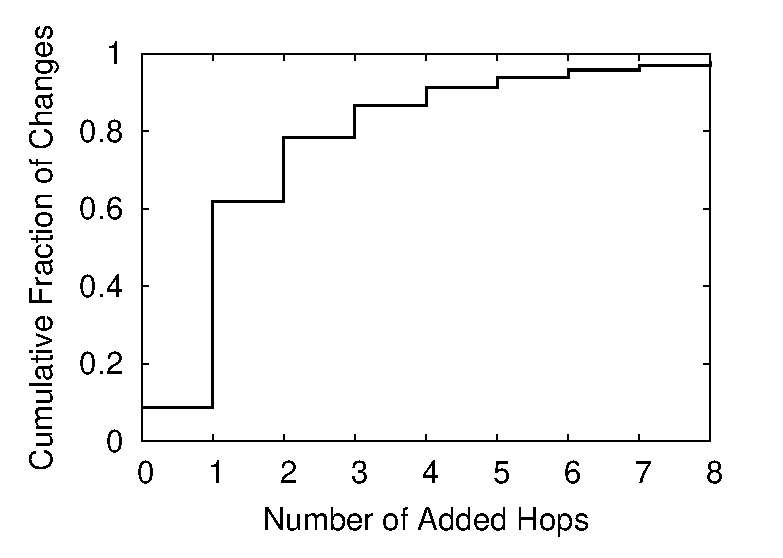
\includegraphics[width=\textwidth]{figs/nadded.eps}
\caption{Number of hops added in path changes.}
\label{fig:char.nrouters}
\end{minipage}
\hfill
%
\begin{minipage}{0.32\textwidth}
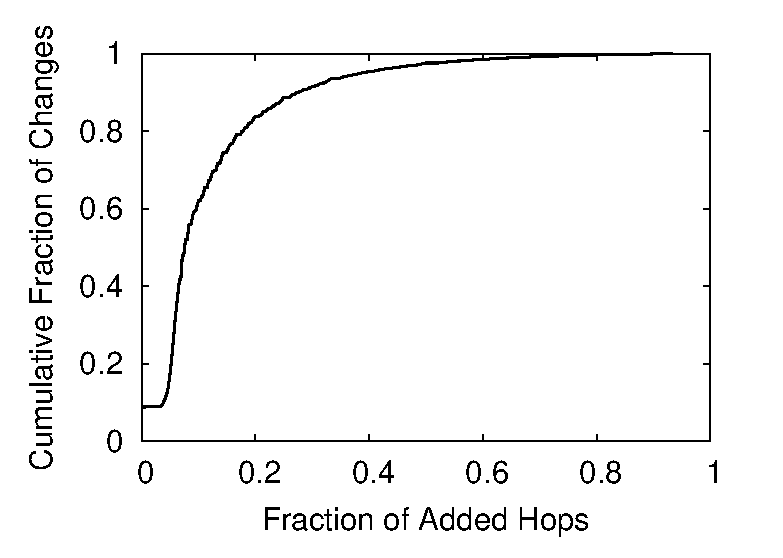
\includegraphics[width=\textwidth]{figs/fracsadded.eps}
\caption{Fraction of hops added in path changes relative to new route
length.}
\label{fig:char.fracs}
\end{minipage}
\hfill
%
\begin{minipage}{0.32\textwidth}
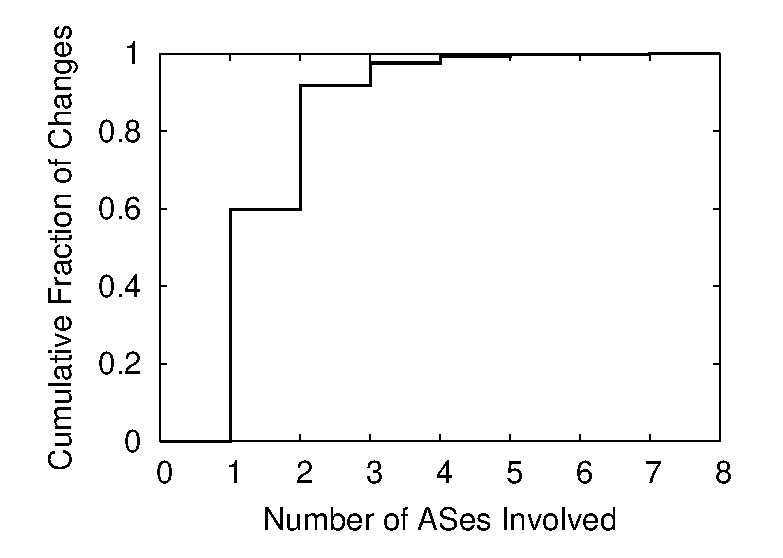
\includegraphics[width=\textwidth]{figs/nasns.eps}
\caption{Distribution of the number of ASes involved in path changes.}
\label{fig:char.nasns}
\end{minipage}
%
\end{figure*}

%  % OLD IMC SETUP WITH 2 FIGS ONLY.  FIGS 1--3 FROM SEC. 3
%  \begin{figure}[t]
%  %\begin{minipage}{0.33\textwidth}
%  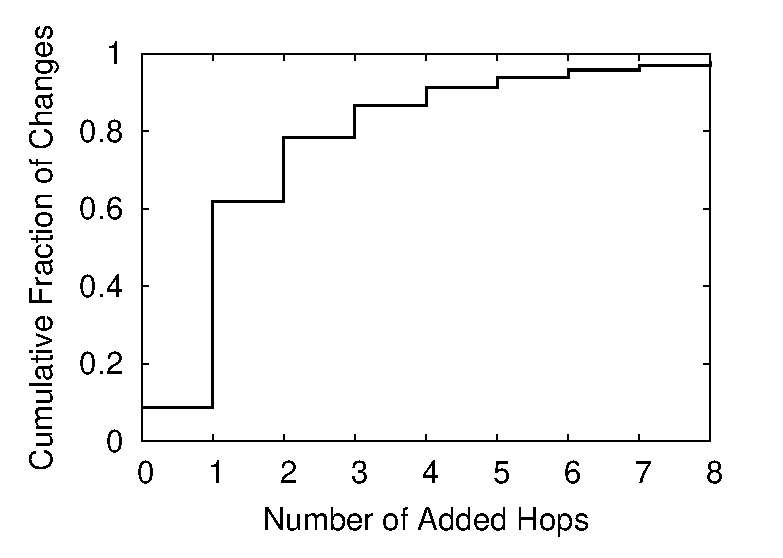
\includegraphics[width=\columnwidth]{figs/nadded.eps}
%  \caption{Number of hops added in path changes.}
%  \label{fig:char.nrouters}
%  %\end{minipage}
%  %\hfill
%
%  %\begin{minipage}{0.33\textwidth}
%  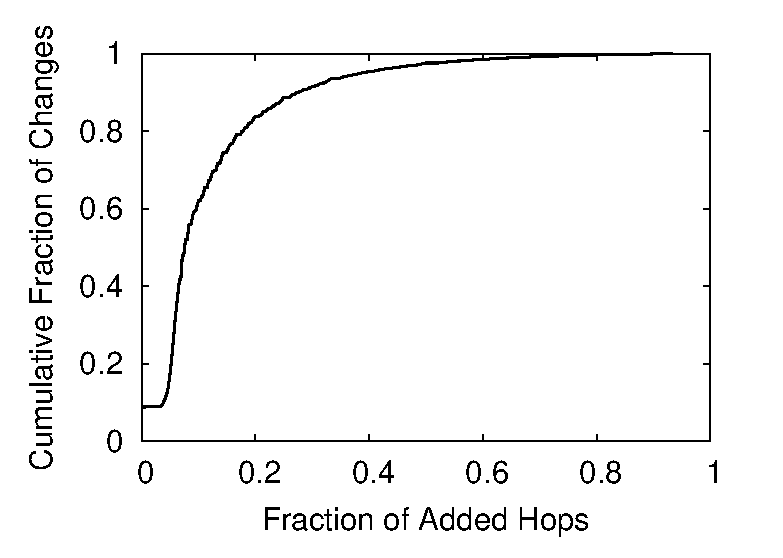
\includegraphics[width=\columnwidth]{figs/fracsadded.eps}
%  \caption{Fraction of hops added in path changes.}
%  \label{fig:char.fracs}
%  \end{figure}
%  %\end{minipage}
%  %\hfill
%  %\begin{minipage}{0.33\textwidth}
%  %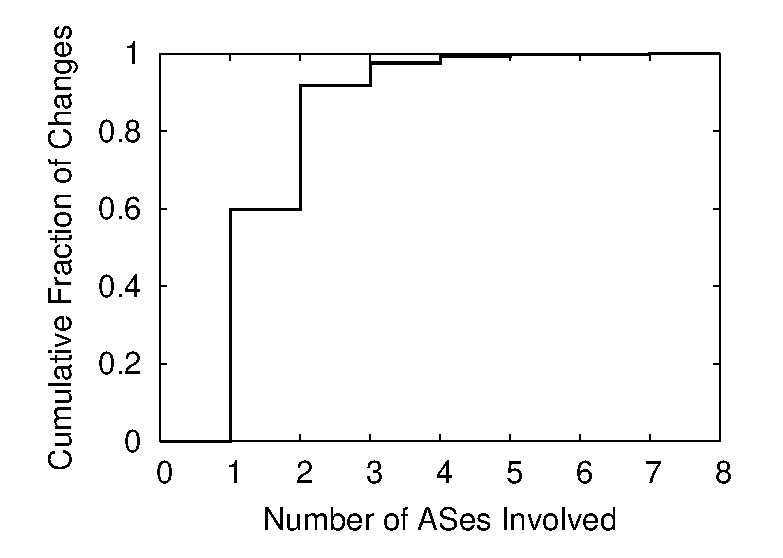
\includegraphics[width=1.05\textwidth]{figs/nasns.eps}
%  %\caption{Distribution of the number of ASes involved in path changes.}
%  %\label{fig:char.nasns}
%  %\end{minipage}


In this section we establish that most path changes involve few hops.
We deployed \dtrack{}~\cite{cunha11dtrack} (using complete remapping) to
track path changes from 72 PlanetLab nodes for one week starting March
4th, 2011.  Each monitor chose 1,000 destinations randomly from a list
of 34,820 reachable destinations.  We used a probing rate of 8 probes per
second, similar to the rate used by DIMES~\cite{shavitt09dimes}, and
observed 1,202,960  changes.  The observed paths traversed 7,315 ASes,
and 97\% of those with more than 50
customers~\cite{luckie13asrel}.

% \footnotetext{Data sets publicly available at
% www.dcc.ufmg.br/\url{~}cunha/datasets.}

%The number of hops added in a change is $h_c - h_d - 1$, assuming we know the previous route.

\figstr~\ref{fig:char.nrouters} shows the distribution of the number of hops
added by path changes, with one or more local change zones (the number of
removed hops is not shown).  This number represents the minimum number of hops
we need to measure to correctly map the new route.  We see that 78\% of
changed paths add only one or two hops, which is small compared to the median
route length of 16 hops (not shown).  The most common type of path change
(52\%) replaces one hop with another.  We note that 9\% of changes only remove
hops from the old route. This may happen when probe filtering or failures
prevent hop measurement.


% \begin{figure}[t]
% \begin{center}
% 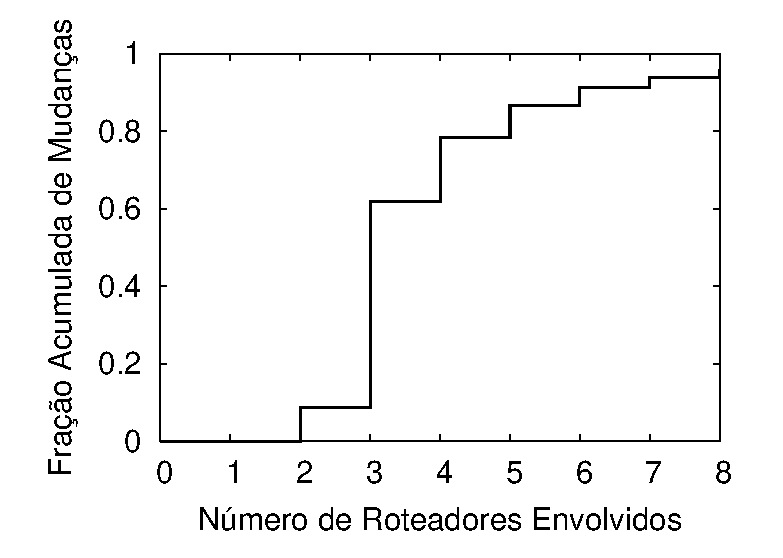
\includegraphics[width=0.8\columnwidth]{figs/nrouters.eps}
% \caption{Distribution of the number of hops involved in path changes.}
% \label{fig:char.nrouters}
% \vspace{-3mm}
% \end{center}
% \end{figure}

% \begin{figure}[t]
% \begin{center}
% 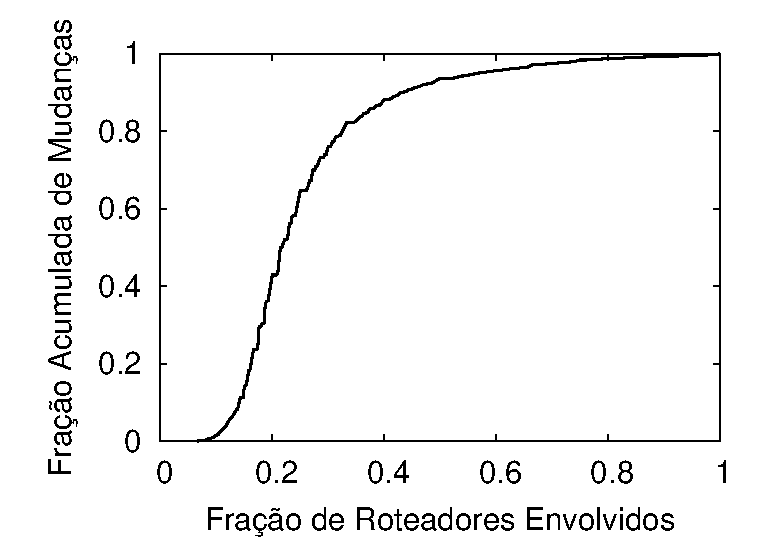
\includegraphics[width=0.8\columnwidth]{figs/fracs.eps}
% \caption{Distribution of the fraction of routers involved in path
% changes.}
% \label{fig:char.fracs}
% \vspace{-3mm}
% \end{center}
% \end{figure}

\figstr~\ref{fig:char.fracs} shows the distribution of the number of
added hops as a fraction of the (new) route length.  The curve is flat
before $x = 0.033 = 1/30$ as \dtrack{} only measures up to 30 hops in a
route (the default in Paris traceroute~\cite{veitch09balancer}).  In
80\% of cases less than 18\% of hops in the new route are new.  This
result shows the potential savings from local remapping compared to
complete remapping.

We translate interface IP addresses measured by \dtrack{} to AS
numbers combining IP-to-AS mapping databases from Team
Cymru\footnotemark{} and iPlane~\cite{madhyastha06iplane}.  IP address
that do not appear in any database are given their own fake AS number,
resulting in overestimation.  \figstr~\ref{fig:char.nasns} shows the
distribution of the number of ASes involved in a given path change.  We
consider an AS to be involved if it contains any interface in a changed
hop.  We find 60\% of path changes are internal to a single AS, and only
7\% involve more than two.  The average number of hops inside each AS in
a route is 3.04.  Similarly, Paxson's seminal work on Internet routing
stability~\cite{paxson97routing} using data collected almost 20~years
ago has shown that paths are significantly more stable at the AS level
than at the IP level.  These facts reinforce the finding that changes
are local and involve few hops.

%\ed{christophe suggested looking at whether paths go back to the
%original routes after two changes.  will keep this in the queue.}

\footnotetext{Team Cymru, IP to ASN Mapping,
{http://www.team-cymru.org/}}
% Services/ip-to-asn.html}}

% \begin{figure}[t]
% \begin{center}
% 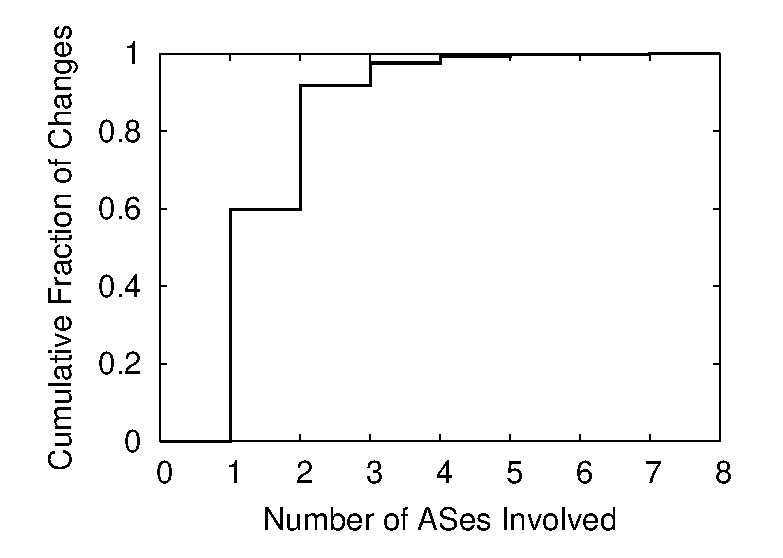
\includegraphics[width=0.8\columnwidth]{figs/nasns.eps}
% \caption{Distribution of the number of ASes involved in path changes.}
% \label{fig:char.nasns}
% \end{center}
% \end{figure}


\section{Local remapping}
\label{sec:remap}

\def\Pi{p_i}
\def\Pii{p_{i-1}}

The local remapping algorithm receives as input the route observed
before the path change, $P(t_{i-1})$, and the radius $r'$ where
\dtrack{} detected a change, i.e., $P(t_i)[r'] \ne P(t_{i-1})[r']$.
Local remapping of this change involves measuring hops on the current
route $\Pi=P(t_i)$, and comparing them with hops on
$\Pii\!=\!P(t_{i-1})$.  A hop is \emph{measured} by sending multiple
probes with systematically varied IP flow-ids, similar to Paris
traceroute's MDA~\cite{veitch09balancer}, to discover the mapping
between interfaces of the measured hop and the hop before it (branch
memberships).

Local remapping operates in two phases:  (i)  locating a $\LCZ$
(\secstr~\ref{sec:remap.locate}), and (ii) remapping it
(\secstr~\ref{sec:remap.local}).  By \emph{locating} a $\LCZ$ we mean
finding a radius $r$ inside it.  If the hop at $r'$ is a changed (added)
hop, then $r'\in\LCZ(r')$ and so $\LCZ(r')$ is already located.


% Local remapping starts from radius $r'$ where the current hop differs
% from the previous one, i.e., $\Pi[r^\prime] \ne
% \Pii[r^\prime]$.  If the hop at radius $r^\prime$ in the current
% route is not contained in the previous route, i.e., $\Pi[r^\prime]
% \notin \Pii$, then radius $r^\prime$ is inside the local change
% zone, no search is necessary, and local remapping proceeds to the next
% phase to locally remap the change (\secstr~\ref{sec:remap.local}).

\subsection{Locating a LCZ}
\label{sec:remap.locate}

Assume for the moment that the only hops which have changed lie in $\LCZ(r')$, so there is
only one $\LCZ$.  By definition if we need to locate it then $r'\ge r_c$.
\figstr~\ref{fig:remap.example} gives an example of this scenario with $r'=6$.
A probe to $r'=6$ detects a path change if the returning packet comes
from interface $I_5$ instead of $\{I_6\} = \Pii[6]$.

To locate the $\LCZ$ we need to find a changed hop.  To do so we perform
a binary search over  $0\le r <r'$.  There are three possible outcomes
and associated conclusions or `rules' for the status of hop $h =\Pi[r]$
found at any $r$ during the search:

%\figstr~\ref{fig:remap.example} shows an example of a path change
%consisting of a single $\LCZ$ where hop $\{I_4\}$ was removed and hops $\{I_8\}$ and $\{I_9\}$
%added.  A probe to $r'=6$ detects a path change as the answer comes
%from $\{I_5\} = \Pi[6]$ instead of $\{I_6\} = \Pii[6]$.

\begin{description}
%
	\item[Rule 1] $h \notin \Pii$ --- conclude $r_d < r <
	r_c$, i.e.~$h$ has changed, and so is inside the local change
	zone.
%
	\item[Rule 2] $h \in \Pii$ and $\Pii\langle h\rangle
	\ne r$ --- conclude $r_c \le r$ since $h$ is unchanged but at
	different radius (hop changes must have occurred upstream).
%
	\item[Rule 3] $h\in \Pii$ and $\Pii\langle h\rangle =
	r$ --- conclude $r \le r_d$ since $h$ is unchanged, no evidence
	of any change upstream, and $\LCZ(r')$ is certainly downstream.
%
\end{description}

The location search initializes variables $r_\mathrm{up} = 0$,
$r_\mathrm{down} = r^\prime$.  At each iteration the hop at radius $r =
(r_\mathrm{up} + r_\mathrm{down})/2$ is measured and the appropriate
`Rule' applied.  Under Rule 3 we set $r_\mathrm{up} = r$; under Rule 2
we set $r_\mathrm{down} = r$.  Rule 1 implies we have located a local
change zone, so the location search is terminated and we proceed to the
actual remapping.



%The algorithm applies the following three rules after measuring hop $h =\Pi[r]$:


% Local remapping initializes $r_\mathrm{up} = 0$ and $r_\mathrm{down} =
% r^\prime$.  At each iteration in the search, local remapping measures
% the hop at radius $r = (r_\mathrm{up} + r_\mathrm{down})/2$ and
% proceeds as follows:

% If the previous route contains the hop at radius $r^\prime$ at a
% different radius $r''$, i.e., $\Pi[r^\prime] = \Pii[r'']$,
% then we have a local path change that added or removed hops to the
% path upstream of $r^\prime$.  \figstr~\ref{fig:remap.example} shows an
% example of one path change where hop $I_4$ was removed and hops $I_8$
% and $I_9$ were added.  A probe to radius six detects a path change as
% the answer comes from $\{I_5\} = \Pi[6]$ instead of $\{I_6\} =
% \Pii[6]$ in the previous route.


\begin{figure}[t] % {{{
\vspace{-7mm}
\begin{center}
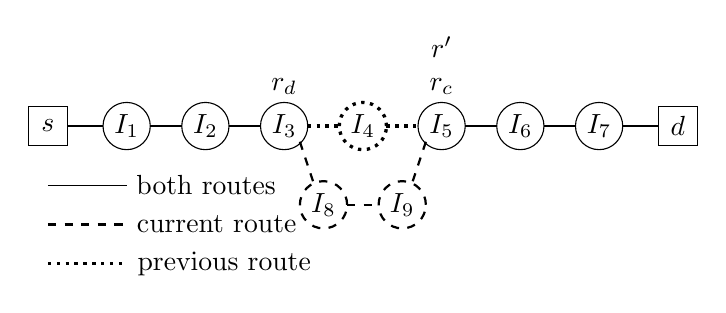
\begin{tikzpicture}
\draw (-2.25,-0.5) -- (-2.25,0) -- (-2.25+0.5,0) -- (-2.25+0.5,-0.5) --
cycle;
\node at (-2,-0.25) {$s$};
%
\draw (6.25-0.5,-0.5) -- (6.25-0.5,0) -- (6.25,0) -- (6.25,-0.5) --
cycle;
\node at (6,-0.25) {$d$};
%
\draw (-1,-0.25) circle (3mm);
\draw (0,-0.25) circle (3mm);
\draw (1,-0.25) circle (3mm);
\draw[dotted, very thick] (2,-0.25) circle (3mm);
%\draw (2,-0.25) circle (3mm);
\draw (3,-0.25) circle (3mm);
\draw (4,-0.25) circle (3mm);
\draw (5,-0.25) circle (3mm);
\node at (-1,-0.25) {$I_1$};
\node at (0,-0.25) {$I_2$};
\node at (1,-0.25) {$I_3$};
\node at (2,-0.25) {$I_4$};
\node at (3,-0.25) {$I_5$};
\node at (4,-0.25) {$I_6$};
\node at (5,-0.25) {$I_7$};
%
\foreach \i in {-1,...,0}
{ \draw (\i+0.3,-0.25) -- (\i+1-0.3,-0.25); }
\foreach \i in {3,...,4}
{ \draw (\i+0.3,-0.25) -- (\i+1-0.3,-0.25); }
\draw[dotted, very thick] (1+0.3,-0.25) -- (2-0.3,-0.25);
\draw[dotted, very thick] (2+0.3,-0.25) -- (3-0.3,-0.25);
\draw (-2.25+0.5,-0.25) -- (-1-0.3,-0.25);
\draw (5+0.3,-0.25) -- (6.25-0.5,-0.25);
%
\draw[dashed, thick] (1.5,-1.25) circle (3mm);
\draw[dashed, thick] (2.5,-1.25) circle (3mm);
\node at (1.5,-1.25) {$I_8$};
\node at (2.5,-1.25) {$I_9$};
\draw[dashed, thick] (1.2,-0.45) -- (1.4,-1.05);
\draw[dashed, thick] (2.8,-0.45) -- (2.6,-1.05);
\draw[dashed, thick] (1.5+0.3,-1.25) -- (2.5-0.3,-1.25);
%
\node at (1, 0.25) {$r_d$};
\node at (3, 0.25) {$r_c$};
\node at (3, 0.75) {$r^\prime$};
%
\draw (-2,-1) -- (-1,-1) node[right] {both routes};
\draw[dashed, thick] (-2,-1.5) -- (-1,-1.5) node[right] {current route};
\draw[dotted, very thick] (-2,-2) -- (-1,-2) node[right] {previous route};
%
\end{tikzpicture}
% \vspace{3cm}
\end{center}
\vspace{-1em}
\caption{Path change removing $I_4$ and adding $I_8$ and $I_9$.}
\label{fig:remap.example}
\end{figure} % }}}

In the general case, where there are other changed hops outside
$\LCZ(r')$, the algorithm may locate another $\LCZ$ to the left of
$\LCZ(r')$ instead of $\LCZ(r')$ itself.

% and looks for hop $\Pi[h]$ on the previous route.
% Again, if hop $\Pi[h]$ is not in the previous route, i.e., $\Pi[h]
% \notin \Pii$, the search finishes and local remapping goes to the
% next phase to remap the change.  If hop $\Pi[h]$ in the current route
% is at radius $h$ in the previous route, i.e., $\Pi[h] =
% \Pii[h]$, then the path change is downstream of $h$ and local
% remapping makes $h_\mathrm{up} = h$.  If hop $\Pi[h]$ is another at
% another radius $h^{\prime\prime}$ in the previous route, i.e.,
% $\Pi[h] = \Pii[h^{\prime\prime}]$, the change is upstream of
% $h$ and local remapping makes $h_\mathrm{down} = h$.

We cannot compare the current route with the previous route if the
router at hop $\Pi[r]$ does not answer probes.  In this case we take a
conservative approach, decrementing $r$ and continuing the search at the
previous hop without updating $r_\mathrm{up}$ and $r_\mathrm{down}$.  If
a path change only removes hops, then all hops in the current route
belong to the previous route.  In this case, the search terminates when
$r_\mathrm{up} = r_\mathrm{down}$.




%%%%%%%%%%%%%%%%%%%%%%%%%%%%%%%%%%%%%%%%%%%%%%%%%%%%%
\subsection{Remapping}
\label{sec:remap.local}

Remapping starts from a radius $r$ of a changed hop inside the located
$\LCZ$, defined by $(r_d,r_c)$.  It sequentially measures hops
downstream of $r$ until it finds the (unchanged) convergence hop
$\Pi[r_c]$.  If one of the branches does not reach $d$, we define the
convergence hop as the last reachable hop, defined as one having three
following unresponsive hops, like in traceroute.  Similarly, local
remapping sequentially measures hops upstream of $r$ as needed until it
finds the (unchanged) divergence hop $\Pi[r_d]$,  terminating at the
source in the worst case.    For path changes that only remove hops, we
have $r_d = r_\mathrm{up} = r_\mathrm{down}=r_c$ at termination and no
remapping is necessary.

The algorithm operates on a principle that it will remap any changes it
becomes aware of in the course of remapping.  Thus if the radius of the
divergence hop $\Pi[r_d]$ has changed, i.e., $r_d \ne \Pii\langle
\Pi[r_d]\rangle$, then this constitutes a detection of other changes, in
particular the existence of another $\LCZ(r_d)$, defined by
$(r_d^1,r_c^1)$ with $r_c^1\le r_d$, upstream of the first.  Similarly,
hops we measured downstream of $r_c$ may have radii incompatible with
the number of hops added or removed by the zone just remapped.  In these
cases, we call the algorithm recursively starting from the radius $r''$
where the new $\LCZ(r'')$ was detected.  This process of remapping
detected changes via $\LCZ$ patches is repeated recursively until there
is no remaining evidence of change.

% \begin{algorithm}[h]
% \caption{Remap phase algorithm (\secstr~\ref{sec:remap.local})
%
% \KwIn{radius $r$ with $r_d < r < r_c$}
%
% % $r_d \leftarrow r$\textbf{,} $r_c \leftarrow r$
%
% % \textbf{while} $\Pi[r_c] \notin \Pii$\textbf{:}
% % $r_c \leftarrow r_c + 1$\textbf{,} measure($r_c$)
%
% % \textbf{while} $\Pi[r_d] \notin \Pii$\textbf{:}
% % $r_d \leftarrow r_d - 1$\textbf{,} measure($r_d$)
%
% \textbf{foreach} $r \in [r_d, r_c]$\textbf{:} measure($r$)
%
% \textbf{if} $r_d \ne \Pii\langle \Pi[r_d]\rangle$\textbf{:}
% search(0, $r_d$)
%
% \textbf{foreach} $r > r_c$ measured\textbf{:}
%
% \Indp
% $h_r \leftarrow \Pi[r]$\textbf{,} $h_c \leftarrow \Pi[r_c]$
%
% \mbox{\textbf{if} $r - r_c \ne \Pii\langle h_r\rangle -
% \Pii\langle h_c\rangle$\textbf{:} search($r_c$, $r$)}
%
% \end{algorithm}



% FIGS. 5--7 FROM SEC. 5
\begin{figure*}
\begin{minipage}{0.33\textwidth}
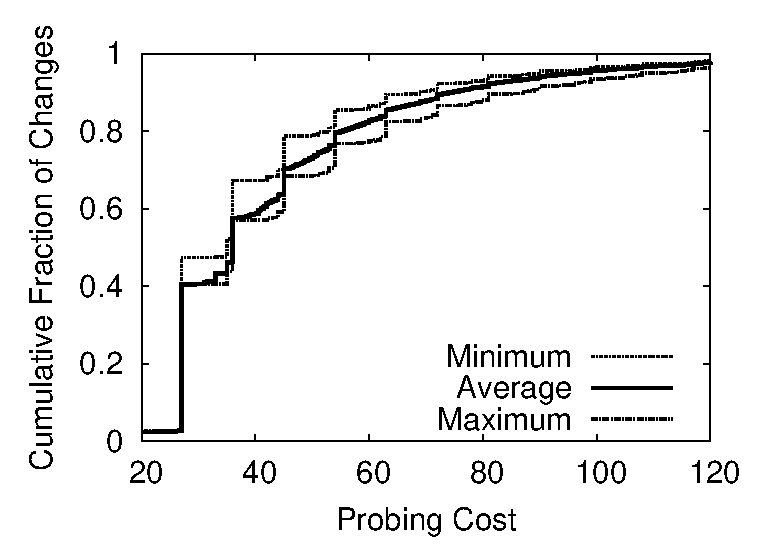
\includegraphics[width=1.05\textwidth]{figs/rmprtcost.eps}
\caption{Probing cost of local remapping over all possible
detection radii.}
\label{fig:sim.rmprt.start}
\end{minipage}
\hfill
\begin{minipage}{0.33\textwidth}
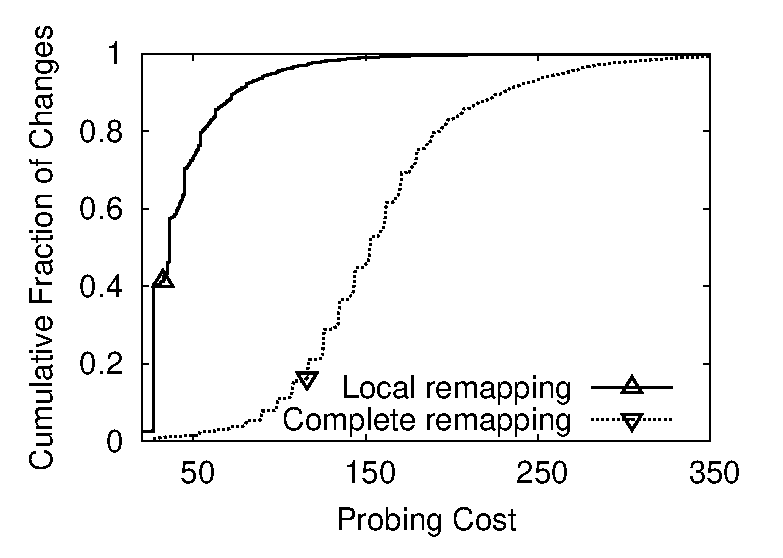
\includegraphics[width=1.05\textwidth]{figs/costprobe.eps}
\caption{Comparing probing cost between local and complete remapping.}
\label{fig:sim.abs.cmp}
\end{minipage}
\hfill
\begin{minipage}{0.33\textwidth}
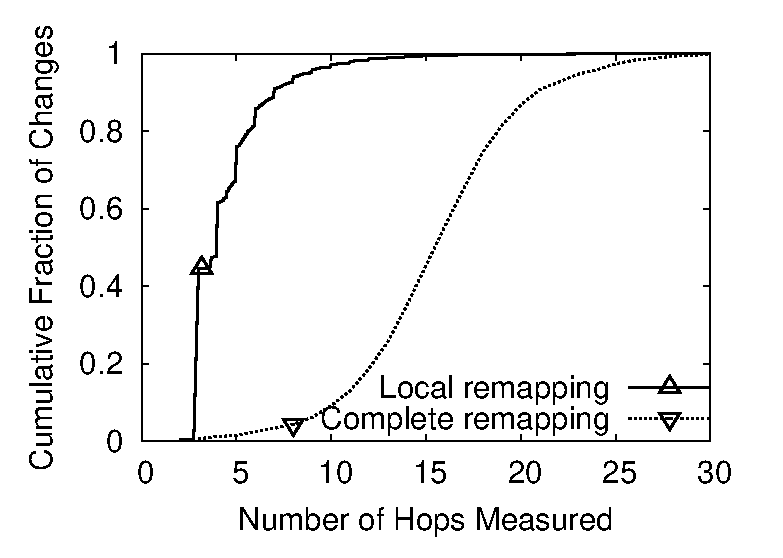
\includegraphics[width=1.05\textwidth]{figs/costhop.eps}
\caption{Comparing number of hops measured during remapping.}
\label{fig:sim.abs.cmp.hops}
\end{minipage}
\end{figure*}


\subsection{Local remapping example}

Consider the path change shown in \figstr~\ref{fig:remap.example}, and
assume it was detected at $r'=6$ as described above.  Since hop $\{I_5\}
=\Pi[r']$ is itself unchanged (existed in $\Pii$), the detection arose
due to the radius being different than expected, 6 instead of 5, and so
$r' \notin \LCZ(r')$ and a location phase is needed.  A binary search is
therefore initiated to locate a change zone.  The search first measures
the hop at $r=r'/2=3$, and finds $\Pii[3] = \Pi[3] = \{I_3\}$,
i.e.~unchanged (and with no evidence of further changes upstream),
indicating that $r_d\ge3$.  Hence Rule 3 applies, and the search then measures
the fourth hop to find $\Pi[4] =\{I_8\}$, which is an added hop (not
in $\Pii$).  Rule 1 now applies:  a $\LCZ$ has been located at $r=4$
(with $r_d$ determined to be $r_d=3$).  The algorithm enters the
remapping phase, measures the fifth hop, and terminates having found
$(h_d,h_c)=(3,5)$ for the located $\LCZ$.  In this case the first $\LCZ$
found is $\LCZ(r')$, the only one in this route.



% \subsection{Serious local remapping example}
%
% Assume a detection at $r'=6$. The associated hop is in the old route at a different radius, so a locating phase is needed.
% Measure $r = 3$ where Rule 2 applies.
% Measure $r = 1$, find $\{I_1\}$, Rule 3 applies.
% Measure $r = 2$, find $\{I_2, I_9\}$, Rule 1 applies.
% Go to local remap and set $(r_d r_c)=(1,3)$.  Find that $\Pi[6] = \{I_5, I_8\}$ is inconsistent with
% the $\LCZ$ we have just remapped: the $\LCZ$ reduced the route length by
% one, but the radius of $\{I_5, I_8\}$ \emph{increased} by 1, implying other changes in the middle.
% Call the algorithm recursively with $r_\mathrm{up} = 3$ and $r_\mathrm{down} = 6$.
% Measure $r = 4$, find $\{I_{10}\}$,  Rule 1 applies, terminate location phase and move to remapping.
% Find $r'_d = 3$ and $r'_c = 6$.  \ed{needs a bit more polishing and checking.}
%
% \begin{figure}[t] % {{{
% \begin{center}
% \begin{tikzpicture}
% \draw (-2.25,-0.5) -- (-2.25,0) -- (-2.25+0.5,0) -- (-2.25+0.5,-0.5) --
% cycle;
% \node at (-2,-0.25) {$s$};
% %
% \draw (6.25-0.5,-0.5) -- (6.25-0.5,0) -- (6.25,0) -- (6.25,-0.5) --
% cycle;
% \node at (6,-0.25) {$d$};
% %
% \draw (-1,-0.25) circle (3mm);
% % \draw (0,-0.25) circle (3mm);
% \draw[dotted, very thick] (0,-0.25) circle (3mm);
% % \draw (1,-0.25) circle (3mm);
% \draw[dotted, very thick] (1,-0.25) circle (3mm);
% \draw (2,-0.25) circle (3mm);
% \draw (3,-0.25) ellipse (3mm and 5mm);
% \draw (4,-0.25) circle (3mm);
% \draw (5,-0.25) circle (3mm);
% \node at (-1,-0.25) {$I_1$};
% \node at (0,-0.25) {$I_2$};
% \node at (1,-0.25) {$I_3$};
% \node at (2,-0.25) {$I_4$};
% \node at (3,+0.0) {$I_5$};
% \node at (3,-0.50) {$I_8$};
% \node at (4,-0.25) {$I_6$};
% \node at (5,-0.25) {$I_7$};
% %
% % \foreach \i in {-1,...,0}
% % { \draw (\i+0.3,-0.25) -- (\i+1-0.3,-0.25); }
% \foreach \i in {3,...,4}
% { \draw (\i+0.3,-0.25) -- (\i+1-0.3,-0.25); }
% \draw[dotted, very thick] (-1+0.3,-0.25) -- (0-0.3,-0.25);
% \draw[dotted, very thick] (0+0.3,-0.25) -- (1-0.3,-0.25);
% \draw[dotted, very thick] (1+0.3,-0.25) -- (2-0.3,-0.25);
% \draw[dotted, very thick] (2+0.3,-0.25) -- (3-0.3,-0.25);
% \draw (-2.25+0.5,-0.25) -- (-1-0.3,-0.25);
% \draw (5+0.3,-0.25) -- (6.25-0.5,-0.25);
% %
% % \draw[dashed, thick] (-0.5,-1.25) circle (3mm);
% \draw[dashed, thick] (0.5,-1.25) ellipse (3mm and 5mm);
% \node at (0.5,-1.0) {$I_2$};
% \node at (0.5,-1.5) {$I_9$};
% \draw[dashed, thick] (-0.8,-0.45) -- (0.3,-1.00);
% \draw[dashed, thick] (1.8,-0.45) -- (0.7,-1.00);
% %
% \draw[dashed, thick] (2.2,-1.25) circle (3mm);
% \draw[dashed, thick] (2.6,-2.0) circle (3mm);
% \node at (2.2,-1.25) {$I_{10}$};
% \node at (2.6,-2.00) {$I_{11}$};
% \draw[dashed, thick] (2.0,-0.55) -- (2.1,-0.95);
% \draw[dashed, thick] (2.25,-1.525) -- (2.50,-1.755);
% \draw[dashed, thick] (3,-0.75) -- (2.70,-1.75);
% %
% % \node at (1, 0.25) {$r_d$};
% % \node at (3, 0.25) {$r_c$};
% % \node at (4, 0.25) {$r^\prime$};
% %
% \draw (3.25,-1.0) -- (4.25,-1.0) node[right] {both routes};
% \draw[dashed, thick] (3.25,-1.5) -- (4.25,-1.5) node[right] {current route};
% \draw[dotted, very thick] (3.25,-2.0) -- (4.25,-2.0) node[right] {previous route};
% %
% \end{tikzpicture}
% % \vspace{3cm}
% \end{center}
% \vspace{-1em}
% \caption{More complex path change.}
% \label{fig:remap.seriousexample}
% \end{figure} % }}}



\section{Trace-driven Evaluation}
\label{sec:sim}

In this section we evaluate \dtrack{} with trace-driven simulations
using the data set described in \secstr~\ref{sec:char}.  We focus
on comparing the probing cost of remapping path changes using complete
versus local remapping.

\subsection{Probing cost}

Local remapping's probing cost varies according to the radius $r^\prime$
where \dtrack{} detected the change.  \figstr~\ref{fig:sim.rmprt.start}
shows the distribution of local remapping's probing cost for the
minimum, average, and maximum costs, calculated over all radii where
\dtrack{} can detect each change.  We see that the distributions of
minimum and maximum costs are similar.  Many path changes add or remove
few hops, so there are few radii where \dtrack{} can detect the path
change and little variation in probing cost.  In the rest of this
section, we use the average cost as local remapping's probing cost.

% \begin{figure}
% \begin{center}
% 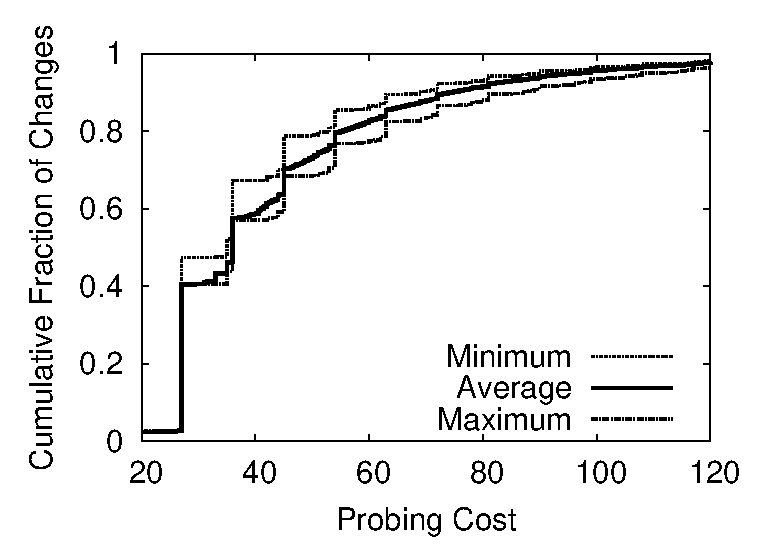
\includegraphics[width=0.8\columnwidth]{figs/rmprtcost.eps}
% \caption{\rmprt{}'s remapping cost varying the hop
% $\boldsymbol{h^\prime}$ where a change is detected.}
% \label{fig:sim.rmprt.start}
% \end{center}
% \end{figure}

\figstr~\ref{fig:sim.abs.cmp} compares probing costs for both local and
complete remapping.  Despite the binary search to locate local change
zones and the need to measure convergence and divergence hops, local
remapping reduces probing costs considerably compared to complete
remapping.  \figstr~\ref{fig:sim.abs.cmp.hops} compares the number of
hops measured by the two approaches.  Comparing with
\figstr~\ref{fig:char.nrouters}, we see that local remapping frequently
measures more hops than the number of added hops, but still only a small
fraction of all hops in a route, shown by the ``complete remapping''
curve.  Local remapping measures at least three hops for 99.6\% of path
changes, even though about 9\% of path changes in our data set only
remove hops from the path (\figstr~\ref{fig:char.nrouters}).  $\LCZ$s
that only remove hops are remapped by the binary search phase of our
algorithm, which takes at least three probes except when $r' < 4$ (which
happens in 0.4\% of path changes in our data).  The remap phase in our
algorithm also measures at least three hops to remap an $\LCZ$: $r_d$,
$r_c$, and changed hops in between.

% \begin{figure}
% \begin{center}
% 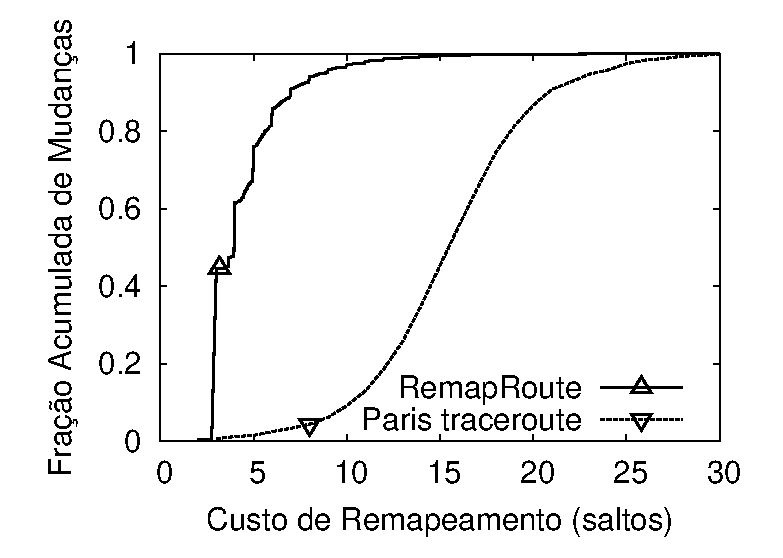
\includegraphics[width=0.8\columnwidth]{figs/costcmp.eps}
% \caption{Comparison of remapping cost between \rmprt{} and Paris
% traceroute.}
% \label{fig:sim.abs.cmp}
% \end{center}
% \end{figure}

\figstr~\ref{fig:sim.savings.cmp} shows the distribution of probing cost
savings when using local remapping instead of complete remapping.  We
compute probing cost savings as $(C_\mathrm{complete} -
C_\mathrm{local})/C_\mathrm{complete}$, where $C_\mathrm{complete}$ and
$C_\mathrm{local}$ are complete and local remapping's probing costs,
respectively.  The solid line, computed for all path changes in our data
set, shows that cost savings are significant.  Local remapping reduces
probing cost by more than half for 88\% of path changes, and reduces the
overall probing cost by 73\%.  The dashed lines in
\figstr~\ref{fig:sim.savings.cmp} show probing cost savings for routes
shorter than 10 hops (labelled ``short'') and routes longer than 20 hops
(labelled ``long'').  Local remapping probing cost savings is higher for
long routes, where complete remapping wastes probes in many hops that
have not changed.

% Local remapping reduces number of hops measured by more than half for
% 88\% of path changes.

\begin{figure}
\begin{center}
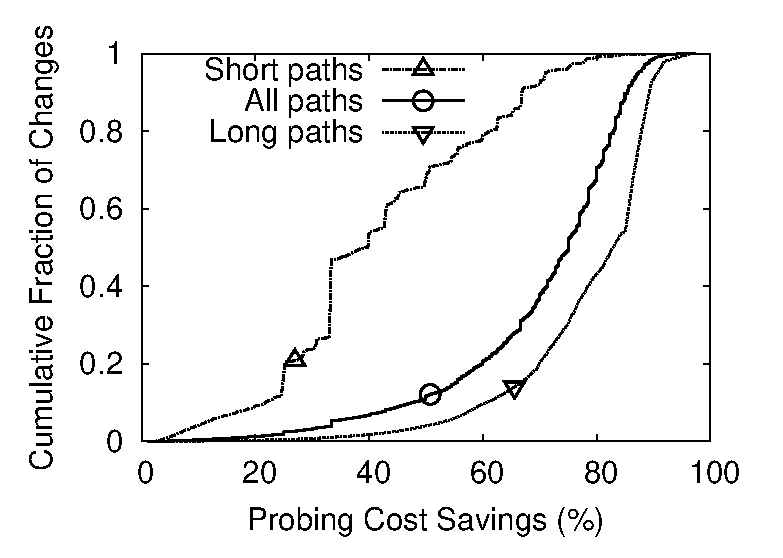
\includegraphics[width=0.8\columnwidth]{figs/probsavings.eps}
\caption{Probing cost savings of local remapping over complete
remapping.}
\label{fig:sim.savings.cmp}
\end{center}
\end{figure}

% FIGS. 9--11 FROM SEC. 6
\begin{figure*}
\vspace{5mm}
\begin{minipage}{0.33\textwidth}
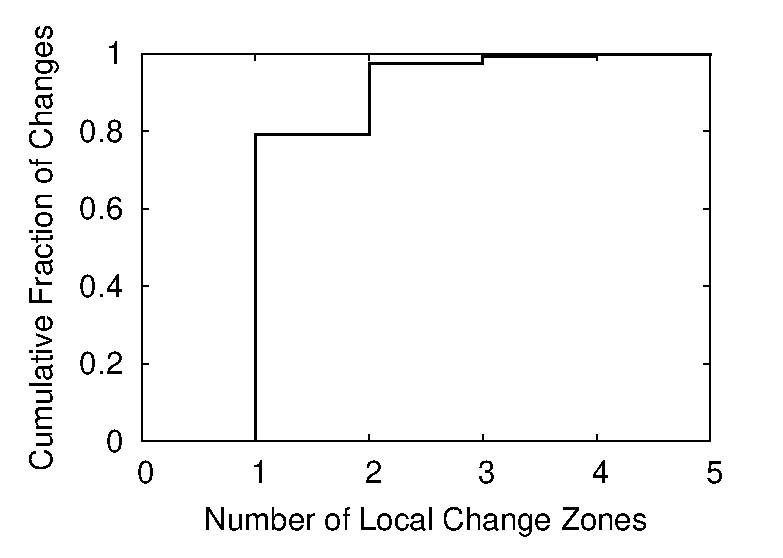
\includegraphics[width=1.05\textwidth]{figs/ndisjoint.eps}
\caption{Number of local change zones in path changes.}
\label{fig:sim.ndisjoint}
\end{minipage}
\hfill
\begin{minipage}{0.33\textwidth}
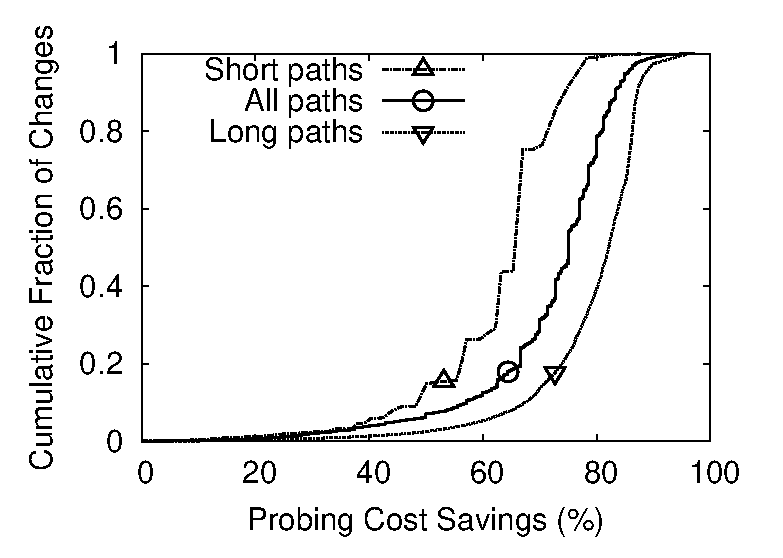
\includegraphics[width=1.05\textwidth]{figs/probsavingsreal.eps}
\caption{Probing cost savings with local remapping in a real
deployment.}
\label{fig:deploy.savings}
\end{minipage}
\begin{minipage}{0.33\textwidth}
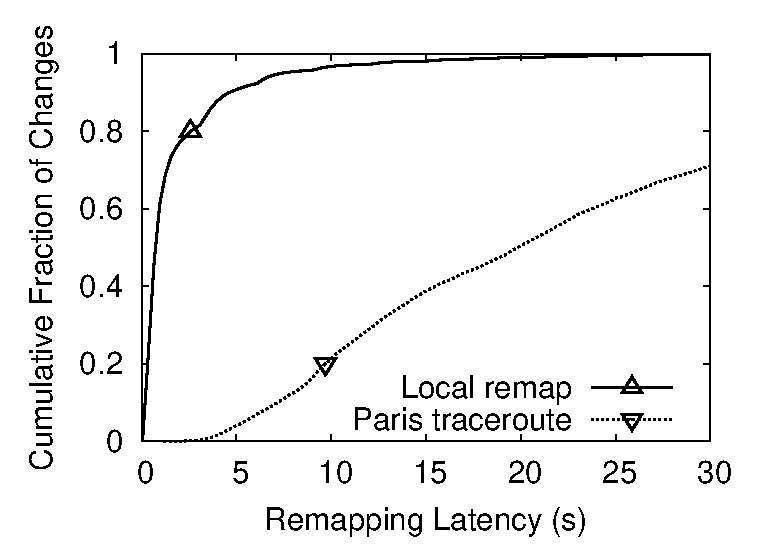
\includegraphics[width=1.05\textwidth]{figs/latencies.eps}
\caption{Comparing remap latency in the real deployment.}
\label{fig:deploy.latency}
\end{minipage}
\end{figure*}

\subsection{Remapping errors}
\label{sec:remap.errors}

Local remapping may only remap parts of a path change when it is
composed of multiple $\LCZ$s.  For example, a route
$p_{i-1} = [s, I_1, I_2, I_3, I_4, I_5, d]$ may change to $p_i =[s, I_1, I_6, I_3, I_9, I_5, d]$.  
In this case there are two local change zones at $(r_d,r_c)=(1,3)$ and $(r_d,r_c)=(3,5)$,
which  \dtrack{} could detect for example as $\LCZ(r'=2)$ or $\LCZ(r'=4)$. 
Local remapping could remap either depending on where the change was detected.

% \begin{minipage}{0.33\textwidth}
% 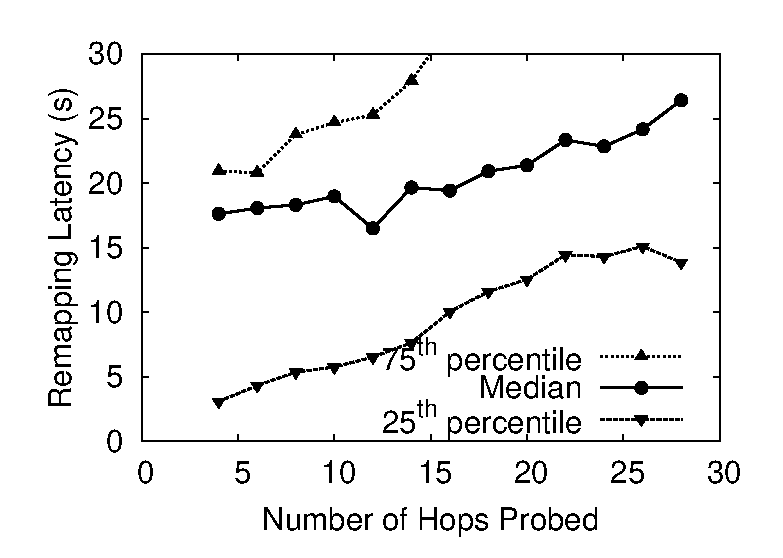
\includegraphics[width=1.05\textwidth]{figs/ptrlatency.eps}
% \caption{Paris traceroute remap latency in the real deployment.}
% \label{fig:deploy.latency.ptr}
% \end{minipage}


To evaluate the prevalence of this problem,
\figstr~\ref{fig:sim.ndisjoint} shows the distribution of the number of
local change zones for consecutive path measurements in our data
set.\footnotemark{}  We observe a single $\LCZ$ in 79\% of cases; here
local remapping, just like complete remapping, will return the correct
new route regardless of detection radius $r'$ (up to statistical errors
in MDA's load balancer discovery).

% , indicating that local remapping will correctly discover the new
% route in most cases.

\footnotetext{We only measure paths when a change is detected, hence all consecutive measurements
observe at least one local change zone.}

Three other factors contribute to minimize the impact of multiple local
change zones.  First, local remapping may remap multiple
$\LCZ$s in one run.  The probability that local remapping will remap 
multiple $\LCZ$s upstream of the detection radius in our data set
is 43\% (in cases where multiple $\LCZ$s exist, not shown).  Second, an
$\LCZ$ which is not remapped when we run local remapping will be
detected and remapped in the future (assuming the new route is stable
enough).  Any $\LCZ$ that is not remapped causes only a temporary
inconsistency.  Third, probing cost savings obtained with local
remapping can be used to increase probing frequency and reduce the
chance that multiple $\LCZ$s appear.

Another limitation of local remapping is that the binary search
mechanism may fail when the relative order of two hops changes between
the previous and current routes.  An extreme, but illustrative, example
is a change from $p_{i-1} = [s, I_1, I_2, I_3, I_4, d]$ to $p_i =
[s, I_4, I_3, I_2, I_1, d]$.  Only 0.9\% of path changes in our data set
reorder hops.  As hop reordering is rare, we take the conservative
approach of remapping the whole path when we detect it. 

Finally, a change may of course occur during remapping.  
This may cause incorrect measurements regardless of remapping approach.  
In practice, \dtrack{} will correct these errors when it reprobes the path, detects that it has
changed, and consequently remaps it.


\section{Evaluation in PlanetLab}
\label{sec:deploy}

In this section we evaluate \dtrack{} with local remapping in PlanetLab.
We deployed a modified version of \dtrack{} in 95 PlanetLab nodes and
collected measurements for one week starting April 19th, 2014.  Our
modified \dtrack{} runs local remapping and complete remapping whenever
it detects a path change.  As in the data set used in the previous
sections, each PlanetLab node has a detection budget of 8 probes per
second and monitors 1,000 destinations chosen randomly from a list of
34,820 reachable destinations in the Internet.  We observed 1,228,559
path changes.  The observed paths traverse 6291 ASes and 96\% of the
ASes with more than 50 customers~\cite{luckie13asrel}.

\figstr~\ref{fig:deploy.savings} shows probing cost savings when using
local remapping instead of complete remapping in the real deployment.
Comparing with \figstr~\ref{fig:sim.savings.cmp}, the average cost
savings in the real deployment are qualitatively similar to the results
we obtained via simulation (solid lines).  Local remapping reduces
probing cost by more than half for 92\% of path changes in the real
deployment, and reduces overall probing cost by 75\%.  Two factors may
explain why probing savings are slightly higher than in the trace-driven
simulations.  First, the set of paths and the monitoring period are
different.  Second,  \dtrack{} targets more detection probes at the last
radii of paths, whereas in the simulations we distribute detection
probes uniformly over all radii.

% 79\% of path changes have divergence hop in the second half of paths

% IMPROVEMENTS:
%
% log detection radius so we can check whether it has an impact on
% savings and accuracy
%
% choose remaprt paths instead of paris traceroute's so we live with
% temporary remapping errors

% \begin{figure}
% \begin{center}
% 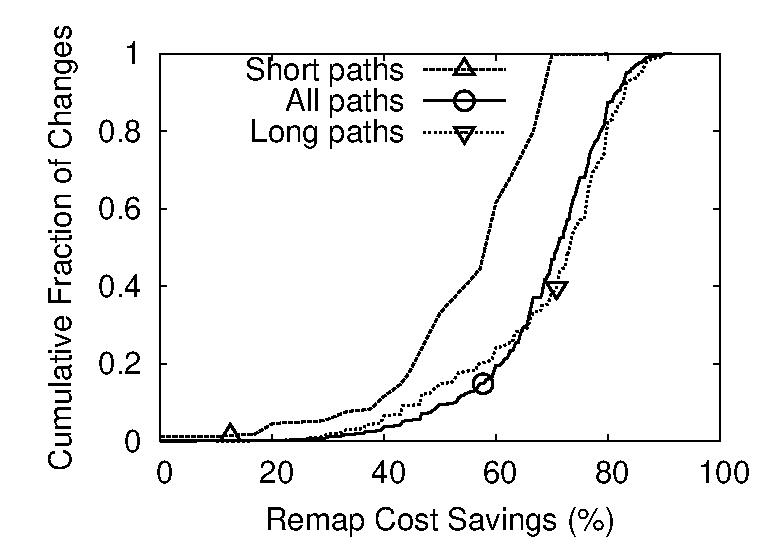
\includegraphics[width=0.8\columnwidth]{figs/deploysavings.eps}
% \caption{Remap cost savings with \rmprt{} in real scenarios.}
% \label{fig:deploy.savings}
% \end{center}
% \end{figure}

% Remap cost savings for short and long routes are more similar to the
% average savings in the real deployment than in the simulations.  In
% other words, the dashed lines in \figstr~\ref{fig:deploy.savings} are
% closer to the solid line than in \figstr~\ref{fig:sim.savings.cmp}.  We
% attribute this change to two factors: (i) the smaller number of observed
% changes may limit the variety of observed changes and (ii) differences
% in the set of monitored paths.\ed{Check text when we get the new
% results.}

\figstr~\ref{fig:deploy.latency} shows the distribution of remapping
latency for local remapping and complete remapping for all changes in
our data sets.  We study latency because local remapping
measures hops sequentially: the next hop to measure is computed based on
the observation at the last measured hop.  Traceroute, however, could
parallelize probing of different hops.  As most path changes require
measuring only a few hops (\figstr~\ref{fig:sim.abs.cmp}), remapping
latency is generally less than 5 seconds.  Complete remapping's
remapping latency is significantly higher, as Paris traceroute's MDA
measures hops sequentially.  We note remapping latency is heavily
affected by implementation choices, but these results show that local
remapping latency is acceptable for use in real systems.  We also note
that \dtrack{} can execute local remapping simultaneously on different
paths if more than one path change is detected in a short time interval.

% \figstr~\ref{fig:deploy.latency} shows the $25^\mathrm{th}$, the
% $50^\mathrm{th}$, and the $75^\mathrm{th}$ percentiles of \rmprt{}'s
% remap latency as a function of the number of hops probed during the
% remapping process.  We studied the remap latency because \rmprt{} probes
% hops sequentially: the next hop to probe is computed based on the result
% of the last probed hop.  Paris traceroute, however, could parallelize
% probing of different hops (but the classic implementation does not).  As
% most \rmprt{} remaps require probing only a few hops
% (\figstr~\ref{fig:sim.abs.cmp}), remapping latency is generally less
% than 5 seconds.  \figstr~\ref{fig:deploy.latency.ptr} shows the
% $25^\mathrm{th}$, the $50^\mathrm{th}$, and the $75^\mathrm{th}$
% percentiles of Paris traceroute's remapping latency in the real
% deployment.  Our objective is not to compare \rmprt{}'s and Paris
% traceroute's remapping latency, as latency is heavily affected by
% implementation choices.  Our objective is to show that \rmprt{}'s
% remapping latency is acceptable for use in real systems.  We also note
% that a topology mapping system like \dtrack{} can execute \rmprt{}
% simultaneously on different paths if more than one path change is
% detected in a short time interval.

% \begin{figure}
% \begin{center}
% 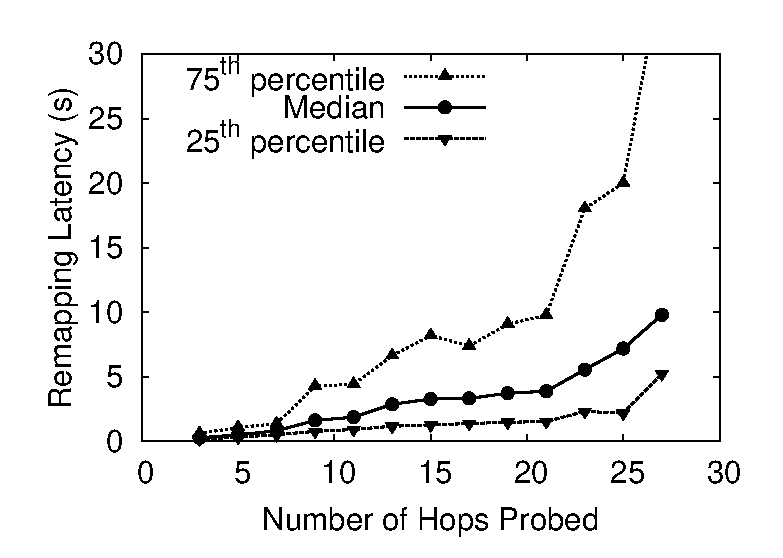
\includegraphics[width=0.8\columnwidth]{figs/latency.eps}
% \caption{RemapRoute remap latency in the real deployment.}
% \label{fig:deploy.latency}
% \end{center}
% \end{figure}

% \begin{figure}
% \begin{center}
% 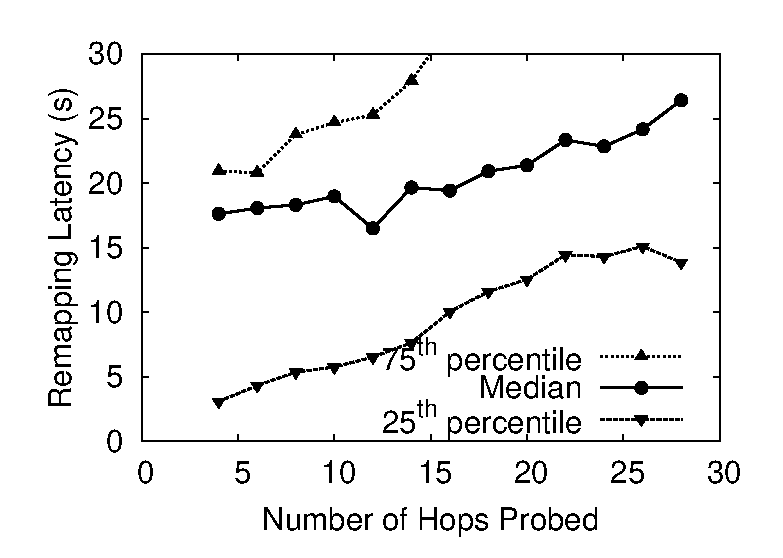
\includegraphics[width=0.8\columnwidth]{figs/ptrlatency.eps}
% \caption{Paris traceroute remap latency in the real deployment.}
% \label{fig:deploy.latency.ptr}
% \end{center}
% \end{figure}

Finally, we also evaluate accuracy, or whether routes measured with
local remapping are equivalent to those measured with complete remapping.
For each observed change in the real deployment, we compare the new
route measured with local remapping and the new route measured with
complete remapping.  We find that local remapping discovers the same
route as complete remapping for 92\% of path changes.  Errors occur
mainly in two cases. In 4.2\% of path changes, local remapping fails to
detect and remap multiple $\LCZ$s. These cases are a limitation local
remapping that results in temporary inconsistencies in the data set
(\secstr~\ref{sec:remap.errors}). In 3.4\% of path changes, local
remapping discovers different branches under load balancing than
complete remapping. The identification of routers that perform load
balancing is probabilistic~\cite{veitch09balancer}.  For example, Paris
traceroute's MDA identifies all interfaces in a path with 95\%
confidence.  Estimation errors are inevitable and cause inference of
different branches regardless of remapping method.  Another cause for
different measurements are path changes that happen during remapping.

% 0.2\% reorderings

In summary, local remapping is almost as accurate as complete remapping,
significantly reduces probing cost, and finishes quickly.


\section{Remapping Routing Events}
\label{sec:patching}

Routing events impact multiple paths in the Internet. Current
monitoring techniques monitor paths independently. Detecting
a routing event on one Internet paths does not trigger any action on
other possibly-impacted paths.  This approach (i) leads to outdated
routing information (as we do not remap paths that have possibly
changed due to the routing events) and (ii) prevents us from
observing the extent of a routing event (as other routing events
might happen before we remap all routes impacted by the first one).
In this section we investigate whether we can use information about
a just-remapped change to quickly detect and remap changes the
underlying routing event caused on other paths.  Our goal is to
develop techniques to efficiently (using few probes) identify and
remap paths impacted by a routing event.

\newcommand{\lczd}{\ensuremath\mathrm{\textsc{lczd}}}

We define a \emph{local change zone domain}, denoted $\lczd(r')$,
for a change detected at radius $r'$ as the hops removed from the
previous path, $p_{i-1}$, around $r'$. More formally, if $r_d$ and
$r_c$ are the radii of the divergence and convergence hops,
respectively, and if $r^\prime_d = p_{i-1}\langle p[r_d]\rangle$ and
$r^\prime_c = p_{i-1}\langle p[r_c]\rangle$ are the radii of the
divergence and convergence hops on the previous route, then
$\lczd(r')$ is defined as the set of hops in $p_{i-1}$ between
$r^\prime_d$ and $r^\prime_c$, i.e., $\lczd(r') = \{p_{i-1}[x]
\mid{} r^\prime_d \le x \le r^\prime_c\}$.

We extended \dtrack{} to evaluate techniques for remapping paths
after detection of a routing event.  Upon detecting a path change at
radius $r'$ on path $p_{i-1}$ (i.e., $p[r'] \ne p_{i-1}[r']$),
\dtrack{} immediately queues path $p_{i-1}$ to be remapped
(remapping starts immediately if there are no ongoing remaps).
After remapping of path $p_{i-1}$ is complete, we compute
$\lczd(r')$. Our extended \dtrack{} then queues all (other)
\emph{overlapping paths} $q$ who intersect $\lczd(r')$, i.e., $q\,
\cap\,\lczd(r') \ne \emptyset$, for remapping (if not queued). It is important to point out that this 
an overlapping path cannot enqueue other overlapping paths once this situation 
originate a recursive loop. Also, to prevent paths that change
overtime and supress other routes to enqueue overlapping paths,
we set a minimum time interval for a path to enqueue overlapping paths
(six hours). 

We deployed the extended \dtrack{} version on 80 PlanetLab nodes useing three 
sources of destinations: TOP100 Alexa,  RIPE Atlas devices and IP addresses from 
different /24 prefixes of  hitlist with 99\% of accuracy. The total number of IP 
addresses were 12763 with a coverage of 5715 ASes in IPlane database. Each PlanetLab selected
1000 random IP address from the list. We allow PlanetLab nodes have overlap
among destinations. The data used in this analysis was colleted between 01/27/2016 
to 03/07/2016, i.e., around 40 days.

Figure~\ref{fig:overlap.delay.cdf} shows the CDF, over all detected
path changes, of the approximate time it takes to remap all
overlapping paths.  Because we remap overlapping paths within
a short period, there is a lower probability that subsequent routing
events will happen while remap is ongoing.
Figure~\ref{fig:overlap.quantity.cdf} shows the CDF, over all
detected path changes, of the fraction of overlapping paths (i.e.,
fraction of other paths that overlap with local change zone
domains).  We observe that 73.68\% of all routes have at least one 
intersection which is a fuel to investigate further if these
overlapping paths also change as well and how the overlapping
interval can help us to detect the change.

\begin{figure}
\begin{center}
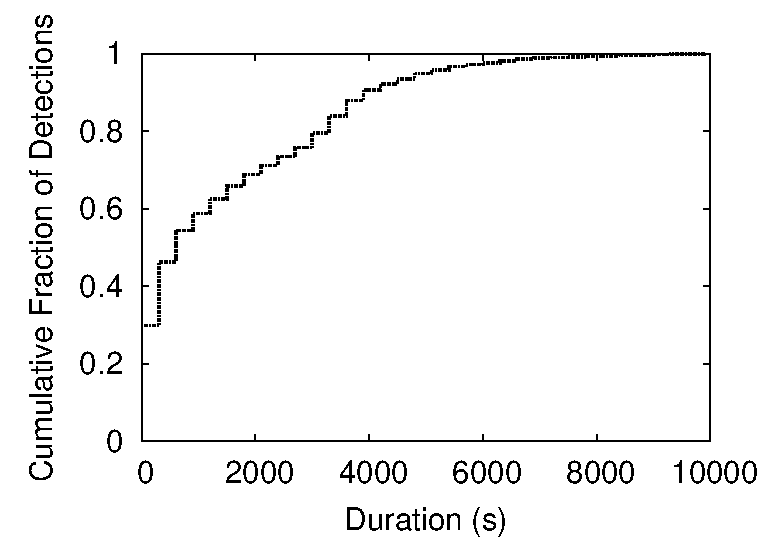
\includegraphics[width=0.8\columnwidth]{figs/patching/durationdetection/durationdetection.eps}
\caption{CDF of detection duration to remap overlappinh routes. }
\label{fig:overlap.delay.cdf}
\end{center}
%
\end{figure}
%
\begin{figure}
\begin{center}
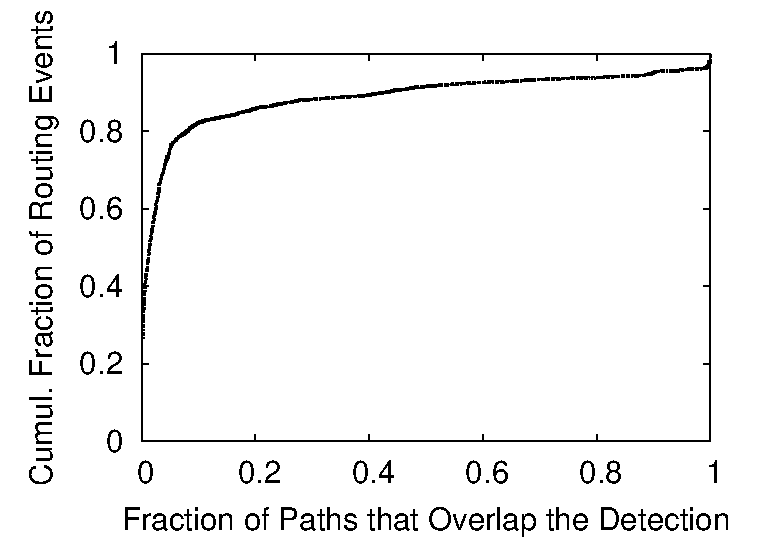
\includegraphics[width=0.8\columnwidth]{figs/patching/routesoverlapping/routesoverlapping.eps}
\caption{CDF of detection overlapping with other routes.}
\label{fig:join.acc}
\end{center}
%
\end{figure}


For each detected path change, we check which of the overlapping
paths have also changed.  Figure~\ref{fig:overlap.change.prob} shows
the fraction of overlapping paths that have changed, grouping
overlapping paths by the fraction of the local change zone domain
that intersects the overlapping paths, i.e.,
$|q\,\cap\,\lczd|\div|\lczd|$.  We note that as overlapping paths
have more in common with the local change zone domain, the higher
the probability that the overlapping path will change.  

\begin{figure}
\begin{center}
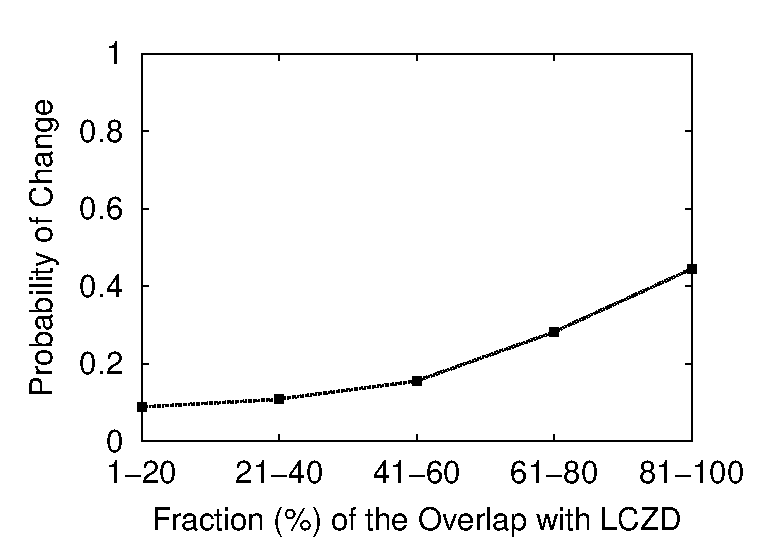
\includegraphics[width=0.8\columnwidth]{figs/patching/probchange/probchange.eps}
\caption{Probability of change given the size of the overlap. }
\label{fig:overlap.change.prob}
\end{center}
%
\end{figure}
%
%We also find
%that paths that have more in common with the path where the change
%was detected have even higher probability of changing (not shown
%\ed{@elverton: but please plot so we can see}).

We now want to find a way to identify whether an overlapping path
has changed (or remained stable).  Let $\lczd'$ denote the local
change zone domain for an overlapping path that has changed, and let
$I = \lczd\,\cap\,\lczd'$ denote the \emph{intersection} of the
local change zone domains for the path where the routing event was
detected ($\lczd$) and an overlapping path ($\lczd'$).
We also define the Candidades Probing Set ($CPS$) as the subpath 
in the overlapping path between the first and last hop in $I$.
We remove the $r_c$ and $r_d$ of $\lczd$, if they are in the overlapping,
once they are not good hops to probe in order to find changes
The data shows that if a $r_d$ is in the intersect, only 0.4\% of times
it changed in the overlapping path. Also, considering that the $r_c$ can
indicate changes when $\lczd'$ have different size, i.e., $|lczd_{p}| \ne l|czd_{p-1}| $ 
we found that the $r_c$ changed only 8.88\% in all intersects such that $r_c \in I$.
For simplicity, we define a $\lczd'_{core}$ as a $\lczd'$ with $r_d$ and $r_c$,
when the last have a $\lczd'$ with equal size, removed.


Figure~\ref{fig:lczd.intersection} shows the distribution of the
number of hops in $CPS$ that are in a $\lczd'$ by the
size of $CPS$,
i.e., $|(CPS \cap \lczd'_{core})| \div |CPS|$.  The distribution shows that 
70,92\% of the $CPS$ does not have any intersection with 
an LCZD' in the overlapping path which 4.83\% of the cases
have an LCZD' that intersections are not capable to detect and 66,09\%
the overlapping path does not change at all. Also, it is clearly that if a 
the $CPS$ intersects a LCZD', probing any hop inside $CPS$ will detect
a change, i.e., in all cases where an overlap crosses an overlapping path
with a change (33,91\% of all intersects), we are able to send a probe into any hop inside
$CPS$ and detect a change with 100\% of precision in 82.89\% of times (28.11\% of all intersections).

%We also looked
%at where the intersection $I$ is located compared to $\lczd$.  We
%find that XX\% of the intersections $I$ are at the start of the
%local change zone (i.e., $r_d + 1$), YY\% of the intersections $I$
%are at the end of the local change zone (i.e., $r_c - 1$), and that
%only ZZ\% of the intersections do are in neither extreme of the
%change zone.


\begin{figure}
\begin{center}
\includegraphics[width=0.8\columnwidth]{figs/patching/overlapcoverage/overlapcoverage.eps}
\caption{Probability of a probe detect a candidates that are in a LCZD on other.}
\label{fig:lczd.intersection}
\end{center}
%
\end{figure}


\section{Related work}
\label{sec:related}

% Operators can use routing protocol logs (e.g., OSPF and IS-IS) and
% router configuration files to map the topology of their
% network~\cite{turner10cenic, markopolou08sprint}.  This approach
% results in accurate and complete topologies, however it is available
% to network operators only and is restricted to a single network.

%We can use public BGP collectors\footnotemark{} and looking glass
%servers to build a map of Internet ASes~\cite{luckie13asrel,
%khan13lookinglass}.  Unfortunately, BGP does not expose all network
%links and public BGP collectors have incomplete AS
%coverage~\cite{oliveira10as2tier}.  AS-level topologies provide limited
%insight about an AS's internal topology.  In this work, we take an
%orthogonal approach and measure the network topology at the interface
%level using active probes.
%
%\footnotetext{The Univ. of Oregon Routeviews Project,
%www.routeviews.org;\newline{}
%RIPE RIS, http://www.ripe.net/data-tools/stats/ris; and others.}

Our work falls in the area of topology mapping with traceroute-style
probing. We can split research on topology mapping according to their
goals: (i) increase Internet coverage, (ii) increase the accuracy of the
measured topology, and (iii) increase measurement frequency.

The usual approach to increase network coverage is to monitor a large
number of paths.  CAIDA's Ark platform~\cite{skitter} attempts to cover
the whole Internet using few monitors to measure paths toward all
reachable $/24$ prefixes.  Unfortunately, Ark takes between two and
three days to measure all these paths due to (unavoidable) bandwidth
limitations at monitors.  An alternative is to share the probing load
among various monitors, like in DIMES~\cite{shavitt09dimes} and
Dasu~\cite{sanchez13dasu}.  These systems can directly use \dtrack{}
with local remapping to reduce network load or increase measurement
frequency.

% In this work, we assume that the sets of monitors and destinations are
% fixed.  However, \dtrack{} does not impose any restrictions on the set
% of monitors and destinations.

Techniques to increase the accuracy of the measured topology perform
more sophisticated probing.  Paris traceroute's Multipath Detection
Algorithm (MDA), for example, sends additional probes systematically
varying values of IP header fields to identify all routers that perform
load balancing in a path~\cite{veitch09balancer}.  \dtrack{} with local
remapping uses Paris traceroute's MDA algorithm to detect load
balancing.  Other tools combine traceroute with IP alias
resolution~\cite{gj13pamplona, keys13midar}, IP Record Route
probes~\cite{sherwood08discarte}, or DNS records~\cite{ferguson13dns} to
build router-level topologies.  These and other techniques send
additional probes per interface of a route and thus increase topology
mapping cost.  By identifying the few hops that have changed, local
remapping can reduce probing cost and increase probing budget available
to perform these more costly (re)mapping techniques at larger scale.

Our work is more closely related to techniques that aim at increasing the
frequency of Internet topology mapping. To increase measurement
frequency we must reduce the probing cost of each path measurement or
the number of monitored paths.  RocketFuel, for example, reduces the
cost to measure a target AS's topology by probing only one of the set of
paths that enter and exit the AS's network through the same border
routers~\cite{spring02rocketfuel}.  Another approach is to reduce the
number of destinations and probe only a single subnetwork in an
AS~\cite{beverly10hifreq}.  Tracetree~\cite{latapy08radar} assumes that
the topology from a monitor to a set of destinations is a tree so it can
eliminate redundant probes to interfaces close to the monitor.
DoubleTree reduces redundant probes to interfaces close to the monitor
(traversed by multiple paths from that monitor) and interfaces close to
the destinations (traversed by paths from different monitors toward the
same destination)~\cite{donnet05topology}. The tree assumption of
Tracetree and DoubleTree, however, is invalid in cases of load balancing
as well as under some traffic-engineering and peering practices. In
fact, our previous work~\cite{cunha11dtrack} shows that Tracetree
detects a very large number of false path changes, which \dtrack{} correctly
identifies as load balancing. \dtrack{} with local remapping reduces
probing cost by focusing on remapping only the parts of the route that
have changed while ensuring route accuracy due to its use of Paris
traceroute's MDA.




\section{Conclusões e trabalhos futuros}
\label{sec:conc}

A manutenção de mapas completos e atualizados da Internet é difícil
devido à grande quantidade de sondas necessárias e restrições de banda
nos monitores.  Neste trabalho propomos o \rmprt{}, uma ferramenta para
reduzir o custo de remapeamento de mudanças de roteamento na Internet.
Dadas a rota anterior a uma mudança de roteamento e um salto
(\emph{hop}) onde a mudança foi detectada, o \rmprt{} (1) realiza uma
busca binária pelo salto onde a mudança aconteceu e (2) faz o
remapeamento local da mudança.  Comparado com a abordagem atual de
remapear a nova rota por inteiro usando traceroute, o \rmprt{} reduz
significativamente o número de saltos sondados para remapear mudanças de
roteamento na Internet.  Essa redução de saltos sondados aumenta a
disponibilidade de sondas, potencializando a medição de mais caminhos ou
aumento da frequência de medições.  O remapeamento com \rmprt{} é tão
preciso quanto remapear o caminho inteiro com traceroute, e a latência
de remapeamento é satisfatória para utilização do \rmprt{} em sistemas
reais.  \rmprt{} é mais um passo na construção de mapas da topologia da
Internet mais completos e atualizados.

Como trabalho futuro, pretendemos integrar o \rmprt{} no \dtrack{} e
prover um serviço de mapeamento da Internet aberto para disponibilizar
informações sobre a topologia para pesquisadores e aplicações.  Queremos
também reduzir ainda mais o custo de remapeamento de mudanças no
\dtrack{}.  Atualmente, o \dtrack{} remapeia cada caminho separadamente.
Esta abordagem desperdiça sondas caso vários caminhos sejam afetados
pela mesma mudança.  Pretendemos desenvolver mecanismos para prever
quais caminhos são afetados por uma mesma mudança e remapear apenas um
deles.




\bibliographystyle{plain}
\bibliography{references}

\end{document}
